% CURE-Rec manuscript -- Elsevier elsarticle template for
% Expert Systems with Applications (ESWA). Numbered reference style.
% Compile: pdflatex cure-rec-eswa; bibtex cure-rec-eswa; pdflatex x2.
% The manuscript deliberately separates controlled causal claims (CURE-Sim)
% from external chronological-ranking claims (MovieLens-1M).

\documentclass[review]{elsarticle}

\journal{Expert Systems with Applications}

\usepackage{graphicx}
\usepackage{multirow}
\usepackage{amsmath,amssymb,amsfonts}
\usepackage{amsthm}
\usepackage{mathrsfs}
\usepackage[title]{appendix}
\usepackage{xcolor}
\usepackage{textcomp}
\usepackage{booktabs}
\usepackage{tabularx}
\usepackage{longtable}
\usepackage{algorithm}
\usepackage{algpseudocode}
\usepackage{array}
\usepackage{placeins}
\usepackage{tikz}
\usetikzlibrary{positioning,arrows.meta}
\hypersetup{hypertexnames=false,bookmarksdepth=3}

\theoremstyle{plain}
\newtheorem{theorem}{Theorem}
\newtheorem{proposition}[theorem]{Proposition}
\newtheorem{corollary}[theorem]{Corollary}
\theoremstyle{definition}
\newtheorem{definition}{Definition}
\newtheorem{example}{Example}
\theoremstyle{remark}
\newtheorem{remark}{Remark}

\newcommand{\Players}{\mathcal{N}}
\newcommand{\Models}{\mathcal{M}}
\newcommand{\Policy}{\pi}
\newcommand{\BasePolicy}{\pi_0}
\newcommand{\Utility}{V}
\newcommand{\Shap}{\phi}
\newcommand{\E}{\mathbb{E}}
\newcommand{\R}{\mathbb{R}}
\newcommand{\NDCG}{\mathrm{NDCG@10}}
\newcommand{\Recall}{\mathrm{Recall@10}}
\newcommand{\CURE}{\textsc{CURE-Rec}}
\newcommand{\Sim}{\textsc{CURE-Sim}}
\newcolumntype{Y}{>{\centering\arraybackslash}p{0.12\textwidth}}

\raggedbottom

\begin{document}


\begin{frontmatter}

\title{CURE-Rec: Constrained Portfolio Selection for Sequential Recommendation via Fully Enumerated Cooperative Games}

\author[1]{Mouad Louhichi}\corref{cor1}\ead{mouad\_louhichi@um5.ac.ma}
\author[1]{Redwane Nesmaoui}\ead{redwane\_nesmaoui@um5.ac.ma}
\author[1]{Mohamed Lazaar}\ead{mohamed.lazaar@ensias.um5.ac.ma}
\cortext[cor1]{Corresponding author.}
\affiliation[1]{organization={National Higher School of Computer Science and Systems Analysis (ENSIAS), Mohammed V University in Rabat}, city={Rabat}, country={Morocco}}

\begin{abstract}
Recommendation interventions alter the exposure process that generates future feedback, but exploration, diversity, long-tail, repetition-control, and provider-balancing policies are commonly evaluated in isolation even though their transformations can interact, compete for slate capacity, and be required to repair an infeasible base policy. We introduce \CURE{}, a decision layer that represents a bounded library of policy transformations as players in a fully enumerated cooperative game. Coalition values are evaluated under disclosed sequential scenarios, explained using exact Shapley values and pairwise interactions, and optimized subject to relevance, fatigue, provider-disparity, and budget constraints. The planner explicitly distinguishes improvement of a feasible base from repair of an infeasible one and can abstain when no robust improvement is available. Nine controlled regimes verify additive, complementary, redundant, antagonistic, delayed, repair, and misspecified cases. In a 20-seed behavioural study, repeat control is selected in every seed, with mean robust lower improvement $0.29371\pm0.00258$ on the normalized CURE-Sim scale. Joint stress tests produce switches to provider balancing, multi-intervention portfolios, and abstention, while configurations selected by a predeclared disagreement-screening rule expose cases in which singleton or marginal-gain heuristics fail to return a valid repair or miss a beneficial multi-intervention portfolio. Separately, audited MovieLens-1M experiments support the shared chronological ranking implementation but do not validate \CURE{}'s policy-selection effectiveness. \CURE{} therefore provides an auditable exact benchmark and decision framework for small intervention libraries; real-world effectiveness requires randomized interventions or policy logs with exposure and propensity information.
\end{abstract}

\begin{keyword}
Recommender systems \sep Explainable AI \sep cooperative games \sep Shapley value \sep policy intervention \sep multi-stakeholder recommendation \sep robust optimization \sep sequential decision making \sep constrained recommendation
\end{keyword}

\end{frontmatter}

\section{Introduction}\label{sec:introduction}

Recommendation is not only prediction. From the earliest collaborative-filtering systems \cite{resnick1994grouplens,sarwar2001item,linden2003amazon} to modern industrial retrieval-and-ranking pipelines \cite{covington2016youtube,ricci2015recommender}, a deployed policy decides which items receive exposure, exposure changes short-term response and repeated-item fatigue, and the resulting feedback modifies the popularity and behavioural signals used at later decisions. The operational question is therefore not only which item should be ranked first at a single time point. It is also which feasible part of the policy should be changed when the current system over-repeats items, under-serves providers, over-concentrates attention, or fails to explore. Production teams already manipulate repetition caps, exploration slots, long-tail promotion, diversity rerankers, novelty slots, and provider balancing \cite{castells2015novelty,abdollahpouri2019popularity,burke2018multistakeholder}. What is generally missing is a coherent way to evaluate their joint long-term consequences and to allocate credit when several interventions are redundant or antagonistic.

A common response is an isolated ablation: activate one intervention, compare a metric with the base policy, and retain the intervention that appears best. Such one-at-a-time evidence is widespread in industrial reporting and in the academic literature on individual re-ranking objectives \cite{ziegler2005improving,vargas2011rank,abdollahpouri2019popularity}. It is, however, a weak basis for a portfolio decision. An exploration slot may be useful only after a repeat cap releases a position; long-tail and novelty slots can compete for the same bounded insertion capacity; a provider correction may be warranted because the base policy violates a platform constraint even if it does not maximize an unconstrained utility increment. Isolated effects do not sum to the value of a portfolio, and a high attribution score alone does not identify a feasible decision.

More precisely, several capabilities are not usually emphasized \emph{jointly} in representative formulations: coalition-level interaction modelling under a shared long-horizon environment, hard feasibility constraints, explicit repair semantics when the base policy is constraint-infeasible, and exact rather than sampled attribution. Table~\ref{tab:capability-gap} positions this combination; it does not claim that no method in a broad research family could be extended to provide a listed capability.

\begin{table*}[t]
\caption{Capabilities emphasized in representative formulations of related approach families. Entries describe the primary object of the cited formulations, not an impossibility result for the broader family. \CURE{} combines the listed capabilities for a bounded intervention library.}\label{tab:capability-gap}
\centering
\scriptsize
\setlength{\tabcolsep}{4pt}
\begin{tabularx}{\textwidth}{@{}>{\raggedright\arraybackslash}X*{5}{Y}@{}}
\toprule
Approach family & Coalition interactions & Long horizon & Hard constraints & Repair semantics & Exact attribution\\
\midrule
Isolated ablations / single-objective reranking \cite{ziegler2005improving,vargas2011rank,abdollahpouri2019popularity} & Not primary & Sometimes & Not typical & Not explicit & No\\
Multi-stakeholder and fairness reranking \cite{burke2018multistakeholder,singh2018fairness,ekstrand2022fairness} & Sometimes & Sometimes & Often & Not explicit & No\\
Off-policy and counterfactual evaluation \cite{swaminathan2015counterfactual,joachims2017unbiased,kallus2020efficient} & Extensible & Yes & Sometimes & Not primary & No\\
Feature/data Shapley attribution \cite{lundberg2017shap,rozemberczki2022shapley} & Sometimes & Not primary & Not primary & No & At small scale\\
\CURE{} (this paper, bounded library) & Yes & Yes & Yes & Yes & Yes\\
\bottomrule
\end{tabularx}
\end{table*}

\CURE{} addresses this gap with a fully enumerated cooperative game over \emph{policy interventions}. Its six players are predeclared slate transformations rather than users, items, model features, or arbitrary retraining operations. A coalition applies a deterministic canonical composition to a fixed base policy. For each coalition and each disclosed sequential scenario, \Sim{} rolls out a finite-horizon platform process with preference, popularity feedback, repeated exposure, fatigue, novelty, and provider exposure. The resulting coalition table supports exact Shapley attribution, exact pairwise interaction analysis, and a direct constrained portfolio decision. Attribution explains a decision; it never replaces the decision rule.

Throughout the paper, \emph{robust} means maximin performance over a finite, disclosed scenario set. \emph{Exact} means that all $2^n$ coalition values in the bounded library are evaluated and the cooperative quantities are computed without subset-sampling error, conditional on that scenario model. Neither term implies that the scenario set exactly represents a deployment environment.

The paper makes four contributions organized around this decision layer.
\begin{enumerate}
\item \textbf{Formalization.} We define a characteristic function over executable policy transformations, including canonical composition, eligibility, collision allocation, deterministic ties, no-op semantics, and declared costs.
\item \textbf{Decision rule.} We select directly from the feasible coalition table using finite-scenario maximin utility and explicitly distinguish improvement, repair, abstention, and the absence of any feasible portfolio.
\item \textbf{Explanation.} We compute exact Shapley values and pairwise interactions from the same coalition table, including a direct attribution of the planner's maximin game, without using attribution scores as the optimizer.
\item \textbf{Evaluation design.} Controlled regimes, behavioural stress tests, selector-disagreement cases, objective and constraint sensitivity, scalability diagnostics, learned-base-policy integration, and a separate MovieLens ranker audit test distinct parts of the framework while preserving their evidence boundaries.
\end{enumerate}

The central claim is deliberately bounded. \CURE{} provides causal-oracle and behavioural claims inside \Sim{}, where the sequential data-generating mechanisms and intervention values are disclosed. It provides real-data ranking claims on MovieLens-1M under an audited evaluator. It does not claim that MovieLens identifies the long-run causal effects of production policy changes: it contains neither logged slates, exposure propensities, nor a complete candidate-set record. This separation is a methodological requirement rather than a limitation hidden in the evaluation.

The remainder of the paper reviews related work, defines the game and decision semantics, presents the evaluation protocols and results, and closes with implications, threats to validity, and reproducibility details.

\section{Literature review}\label{sec:literature}

\subsection{Recommendation as a sequential intervention problem}

Collaborative filtering and sequential recommendation are usually introduced as supervised ranking problems, from probabilistic and regularized matrix factorization \cite{mnih2008probabilistic,koren2009matrix} and Bayesian personalized ranking \cite{rendle2009bpr,pan2008oneclass} to neural collaborative filtering \cite{he2017ncf}, recurrent and self-attentive sequence models \cite{hidasi2016gru,kang2018sasrec,sun2019bert4rec}, and graph-based methods \cite{wang2019ngcf,he2020lightgcn}. These models are powerful predictors, but prediction quality does not by itself decide whether a platform should increase exploration, reduce repetition, or rebalance exposure. A recommendation is an action that changes the observations on which future training and ranking depend. This closed loop motivates causal recommender work and counterfactual learning-to-rank \cite{swaminathan2015counterfactual,joachims2017unbiased,wang2023causal,bonner2018causal}; recent surveys systematize this literature and its identification requirements \cite{gao2024causal}. A complementary recent line studies how recommendation feeds back into the ecosystem itself: user--creator feature dynamics can polarize under dual influence \cite{lin2024polarization}, exploration mediates a trade-off between short-run user satisfaction and long-run creator productivity \cite{yao2024satisfaction}, and platform participants can strategically act on the training data \cite{baumann2024collective}. These results reinforce the premise of the present paper---exposure decisions have long-horizon, multi-sided consequences---while also illustrating why finite-horizon simulator evidence must be labelled as such: our behavioural benchmark discloses one concrete feedback mechanism and does not model strategic creators.

The available evidence often limits what can be inferred. Observational ratings typically record a response but not the alternatives shown, the rank at which they were shown, the logging probability, or the contemporaneous candidate set \cite{pearl2009causality,athey2017state}. Treating such records as complete randomized policy logs conflates preference, exposure, and selection. Work on recommendation as treatment makes this distinction explicit \cite{schnabel2016recommendations}; doubly robust and sequential off-policy approaches require the logging information that ordinary ratings files lack \cite{dudik2014doubly,kallus2020efficient}. \CURE{} follows that discipline: the causal intervention game is tested in an oracle benchmark; the MovieLens experiment remains a separate chronological-ranking robustness evaluation.

\subsection{Diversity, novelty, repetition, and provider exposure}

A long literature improves recommendation lists through diversity, novelty, long-tail exposure, popularity-aware reranking, and multi-stakeholder objectives \cite{ziegler2005improving,vargas2011rank,castells2015novelty,abdollahpouri2019popularity,burke2018multistakeholder,ekstrand2022fairness}. Recent work formalizes the multi-sided dimension of these objectives: item--user fairness can be interpolated through constrained optimization \cite{chen2024interpolating}, and user--item fairness trade-offs admit explicit frontier analyses \cite{greenwood2024fairness}. These contributions usually define one target metric or one re-ranking objective. The operational challenge is that their transformations can collide. A diversity reranker can alter the positions available to a long-tail slot; a novelty slot and a tail slot may propose the same item; and provider balancing can reduce disparity while changing relevance or fatigue. The present work does not replace those objectives. It offers a framework for assessing the exact value of their feasible combinations under a shared platform utility and explicit constraints.

The scope is intentionally modest. The intervention library is not learned from data, and it does not enumerate arbitrary changes to model architecture, user interfaces, retrieval systems, or incentives. These changes would make a coalition ill-defined and destroy exact tractability. Instead, the players are a small set of deployable slate-level transformations with clear costs and collision rules.

\subsection{Cooperative attribution and interactions}

The Shapley value is characterized by the standard efficiency, symmetry, dummy, and additivity axioms \cite{shapley1953}. It has become central to feature attribution \cite{lundberg2017shap,sundararajan2017axiomatic,covert2021understanding} and to broader data and component valuation problems \cite{rozemberczki2022shapley}. When the player set is large, sampling estimators are commonly required \cite{castro2009polynomial}; the bounded intervention library lets us avoid that approximation. Attribution does not itself determine an action: an intervention with a positive Shapley value can still be infeasible, redundant with a lower-cost substitute, or inappropriate when the base policy is already constraint-feasible. We therefore use exact Shapley values to explain coalition values and pair them with direct constrained selection.

Pairwise interaction measures make the non-additivity visible. The Grabisch--Roubens interaction index distinguishes complementary and antagonistic pairs \cite{grabisch1999interaction}; multilinear cooperative extensions offer related representations of coalition effects \cite{owen1972multilinear}. This is particularly relevant for policy transformations because slots and rerankers are not independent switches. The game is exact here because six interventions yield 64 coalitions per scenario. No Monte-Carlo attribution error is required. When player sets are large, exact enumeration is no longer possible and recent estimators approximate any-order Shapley interactions through weighted least squares or stratified subset sampling \cite{fumagalli2024kernelshapiq,kolpaczki2024svarmiq}; those approximation tools address precisely the regime that the bounded intervention library avoids, and they are the natural route to extending the present framework to larger libraries.

\subsection{Robust decision making under model ambiguity}

Partial-identification and robust-decision traditions caution against optimizing a single convenient causal model when several data-generating mechanisms remain plausible \cite{manski2003partial,rosenbaum2002observational,athey2017state}. In recommender systems, ambiguity can arise from fatigue strength, popularity feedback, delayed novelty benefit, provider exposure dynamics, and policy shift. \CURE{} operationalizes this caution as a finite, disclosed scenario set in the current framework. For a coalition, the relevant object is a lower utility improvement over scenarios, not a point estimate from a favourable scenario. This is an ambiguity stress test, not a claim that a finite scenario ensemble nonparametrically identifies a real-world causal effect.

\subsection{From attribution to deployment planning}

Attribution and deployment solve different optimization problems. An attribution method asks how a specified value should be divided among contributors. A deployment planner asks which action should be taken subject to operational constraints. Confusing the two creates a subtle form of overclaiming. A Shapley value can assign positive credit to an intervention because it improves some coalitions, while a planner should reject it because its cost exceeds a budget, it is redundant with a lower-cost substitute, or it makes a provider-disparity or relevance constraint fail. Conversely, an intervention may be selected as a repair even when its unconstrained utility increment is not the largest, because the current policy is not admissible.

This distinction has precedent in constrained and multi-objective recommendation, where fairness or business requirements are enforced as explicit constraints rather than as attribution scores \cite{wu2023multifr,chen2024interpolating}, but it is rarely made explicit in explanation pipelines. A common practice is to report feature or component importance and then make an informal design recommendation. That recommendation may be reasonable, but its feasibility conditions are usually outside the formal object being evaluated. \CURE{} makes the decision object explicit. The cooperative game produces a complete attribution and interaction report; the planner separately evaluates the same coalition values against declared constraints. The result is more falsifiable: a reader can inspect whether a selected portfolio was truly feasible and whether an alternative had a higher lower utility but failed a constraint.

The constrained optimizer is deliberately simple once coalition values are available: for a six-player library, exhaustive feasible maximin selection is preferable to an approximate optimizer. The methodological contribution is therefore not a new combinatorial optimization algorithm. It is the joint construction of (i) a well-defined characteristic function over executable policy transformations, (ii) exact interaction-aware attribution over the same coalition table, and (iii) explicit improvement/repair semantics under hard constraints.

There is also a practical reason to preserve the separation. Platform constraints differ across deployments. A provider-disparity threshold, intervention budget, or tolerated relevance change may be set by policy, product, or law rather than by a statistical estimator \cite{singh2018fairness,biega2018equity,ekstrand2022fairness,mehrabi2021survey,ge2020causal}. Re-running a small exact game with a changed constraint is transparent; retraining an opaque attribution model or quietly changing a scalarized objective is not. The calibration results in this paper are therefore not merely an uncertainty appendix. They show how the proposed decision changes when the stated operating assumptions change.

\subsection{Evaluation discipline for recommender claims}

Ranking results can be invalidated by small protocol differences, including missing-not-at-random feedback and post-selection evaluation bias \cite{yang2018unbiased,sun2020debiased,cawley2010selection}. Models may receive different candidate sets, test targets may be inadvertently removed as ``unavailable'', seen items may leak into one model's candidates, or a test result may select an epoch or a blend. These problems are especially easy to miss in a comparison between a non-personalized baseline, a matrix-factorization model, and a sequential neural model because their natural implementations expose different interfaces.

The external protocol in this paper fixes the candidate universe before model scoring, following the principle that offline ranking comparisons must not change the retrieval ceiling across methods \cite{cremonesi2010performance,harper2015movielens}. A candidate set contains warm catalogue items not seen by the user in training. All models score exactly this vector; a cold target is counted explicitly rather than converted into an apparently easier warm ranking task. Validation and test are separated: Stage A and Stage B model search write validation rows, the selected configuration is frozen in a manifest, and final test audit is run only after selection. The audit then records candidate cardinalities, target presence, score ordering, pairwise preference checks, and restored checkpoint state. This discipline is not a claim that one benchmark establishes general recommender superiority. It is the minimum required for a credible narrow claim about the implemented comparison.

The same discipline applies to uncertainty. Five seeds are useful for revealing optimization instability and for reporting a range, but they are not five independent real-world datasets. The paper reports means, sample standard deviations, minima, maxima, and paired differences rather than presenting a seed average as a universal effect size. The behavioural studies likewise report all OAT and LHS configurations rather than selecting the ones that favour the proposed planner.

\subsection{Positioning}

\CURE{} differs from conventional re-ranking in its unit of analysis: it evaluates interventions and portfolios rather than individual items. It differs from feature attribution in its players and output: the players are feasible policy changes and the output includes a robust constrained decision. It differs from off-policy evaluation because its primary causal evidence is a controlled sequential oracle environment rather than an assertion that an incomplete ratings dataset identifies a counterfactual policy value. Finally, it differs from a new base-recommender paper: the same intervention-game layer can in principle sit above a transparent simulated policy or a learned ranker, provided that the intervention semantics and evaluation protocol are fixed. Section~\ref{sec:semireal} reports one bounded integration case in which a BPR-MF ranker trained on simulator-logged feedback replaces the hand-crafted base and the selected intervention remains unchanged. The external MovieLens models are audited separately under Section~\ref{sec:external-protocol}; placing an externally trained ranker inside the sequential environment remains future work.

\section{Background and preliminaries}\label{sec:background}

\subsection{Sequential recommendation environment}

Let $\mathcal{U}$ be a user cohort of $|\mathcal{U}|$ users, $\mathcal{I}$ an item catalogue of $|\mathcal{I}|$ items with provider map $\mathrm{prov}:\mathcal{I}\to\mathcal{P}$, $d$ the latent dimension, and $t\in\{0,\ldots,T-1\}$ a decision time. The platform state is
\begin{equation}
 X_t=(P_t,H_t,F_t,Q_t,E_t,G_t),
\label{eq:state}
\end{equation}
where $P_t\in\mathbb{R}^{|\mathcal{U}|\times d}$ is the public profile available to the policy, $H_t\in\mathbb{R}^{|\mathcal{U}|\times d}$ denotes latent preference state used only by the simulator response mechanism, $F_t\in[0,1]^{|\mathcal{U}|}$ is user fatigue, $Q_t\in\mathbb{R}_{\geq0}^{|\mathcal{I}|}$ is item popularity, $E_t\in\mathbb{N}^{|\mathcal{U}|\times|\mathcal{I}|}$ is per-user exposure history, and $G_t\in\mathbb{R}_{\geq0}^{|\mathcal{P}|}$ is cumulative provider exposure. A base policy $\BasePolicy$ returns a ranked slate from a candidate catalogue. The environment then produces response and transition variables,
\begin{equation}
 L_t\sim \Policy(X_t),\qquad Y_t\sim p_m(Y_t\mid X_t,L_t),\qquad X_{t+1}=T_m(X_t,L_t,Y_t,\epsilon_t),
\label{eq:transition}
\end{equation}
for scenario $m\in\Models$. The notation makes clear that a policy change affects both immediate response and later state.

A clarification of the $\sim$ notation is important for the exactness claims below. In the implemented benchmark, the base policy and every coalition transformation are \emph{deterministic conditional on the observable state and a keyed random seed}: for seed $\zeta$, the executed slate is $L_t=\Policy_S(X_t;\zeta)$, and all simulator randomness $\epsilon_t$ (initialization, response draws, tie-breaking perturbations) is drawn from an event-indexed stream keyed by $(\zeta,m,t,u,\mathrm{event})$. The distributional notation in Eq.~\eqref{eq:transition} therefore describes the \emph{class} of environments the framework targets; within one seed, policy stochasticity and simulator stochasticity both resolve to the keyed stream, which is what makes coalition values reproducible and coalition semantics permutation-invariant. A deployment that adds genuine policy stochasticity (for example, randomized slate sampling) would draw it from the same keyed construction; the definitions below do not otherwise change.

The behavioural benchmark uses a cohort-level process with hidden affinity, public-profile noise, repeated exposure, satisfaction-mediated preference drift, item-popularity feedback, and provider exposure. The base ranker uses public-profile similarity and popularity rather than hidden interest. This preserves a meaningful gap between the policy's information and the simulator's outcome mechanism.

Two features of this formulation matter for interpretation. First, the state is not merely an enlarged feature vector. Exposure and provider counts are shared, evolving variables: changing one user's slate can alter the popularity signal used in later ranking and the aggregate provider-disparity outcome. We consequently evaluate a cohort rollout rather than treating each user--item record as an independent supervised observation. Second, the latent-interest component is deliberately hidden from the policy. A policy that could inspect the simulator's response state would turn the benchmark into an oracle ranker and would make intervention results difficult to interpret. The policy receives only public profiles, exposure history, candidate availability, and the current popularity state.

The temporal horizon has a direct scientific role. A short horizon emphasizes the immediate relevance cost of an intervention; a longer horizon can reveal an effect operating through fatigue reduction, provider exposure, or preference drift. This is why horizon is not selected from the outcome but varied explicitly in the calibration studies. The OAT study shows this distinction directly: lowering the horizon to eight reduces the mean robust lower improvement to $0.14397$, while increasing it to sixteen raises it to $0.37785$. A one-step ranking evaluation cannot express this trade-off.

\subsection{Evidence, interventions, and causal scope}

A causal claim needs more than a timestamped interaction table. For a real policy evaluation, the analyst would need at least the candidate set available at each decision, the displayed slate and positions, the logging or assignment probability, policy identifiers, a representation of eligibility and inventory, and outcomes at the time scale of the claimed effect. Without these fields, the observed response is confounded by which alternatives were exposed and by which policy generated the exposure. The absence of these fields is not repaired by fitting a more flexible predictor.

This paper therefore uses three evidence layers. The first is an \emph{analytic oracle} layer, where coalition values and true optima are defined transparently. The second is a \emph{behavioural oracle} layer, where the sequential mechanisms in Eqs.~\eqref{eq:state}--\eqref{eq:transition} generate the long-run outcome. The third is an \emph{external ranking} layer, where MovieLens-1M checks the recommender training and evaluation protocol. The layers complement one another but are not interchangeable. Controlled oracle evidence tests whether the cooperative and decision machinery reacts correctly to known structures. Behavioural evidence tests whether those mechanisms remain meaningful under feedback and fatigue. External ranking evidence tests whether the trained ranking models improve an audited held-out metric. Only the first two layers support the paper's causal intervention statements.

The player definition is also causal in a restricted but operational sense. A player is a policy transformation that can be applied while holding the base policy, candidate universe, and intervention semantics fixed. We do not define players as arbitrary features that happen to correlate with response, nor as unrestricted retraining operations. This restriction makes the intervention $do(\Policy\leftarrow\Policy_S)$ interpretable: the system replaces the deployed slate transformation with a declared alternative and executes the same sequential environment. It also makes negative results interpretable. If an intervention has no eligible candidate at a time step, it performs no operation and the event is logged. A no-op is not silently converted into another intervention.

\subsection{Policy transformations as players}

The player set is
\begin{equation}
 \begin{aligned}
 \Players=\{&\texttt{repeat\_cap},\texttt{explore\_slot},\texttt{tail\_slot},\\
              &\texttt{diversify},\texttt{novel\_slot},\texttt{provider\_balance}\}.
 \end{aligned}
\label{eq:players}
\end{equation}
A coalition $S\subseteq\Players$ is a policy transformation, not a set of independently trained models. To avoid permutation-dependent semantics, every coalition follows one canonical order: repeated-exposure cap, eligibility filtering, injection allocation, diversity re-ranking, and provider balancing. The three injection players jointly compete for a capacity of two positions. Each proposes eligible items, normalizes its proposal score within its own scale, and an exact small assignment resolves collisions. A player with no eligible proposal is recorded as a no-op rather than being silently replaced by a popular item. Table~\ref{tab:players} summarizes the players, membership costs, and operational roles.

This design is important for interpretability. If intervention order changes with Shapley permutations, the same coalition can represent several different policies, making the characteristic function undefined. Shapley permutations average marginal contributions over set order; they must not change the operational definition of a set.

\begin{table*}[t]
\caption{Intervention players, declared membership costs, and fixed operational semantics. Costs and thresholds are configuration values rather than learned coefficients; costs are charged whenever a player belongs to the coalition, including steps at which the player records a no-op (Definition~\ref{def:cost}).}\label{tab:players}
\centering
\small
\setlength{\tabcolsep}{3pt}
\begin{tabularx}{\textwidth}{@{}p{0.14\textwidth}c X X@{}}
\toprule
Player & Cost $c_i$ & Slate transformation & Interaction and feasibility relevance\\
\midrule
Repeat cap & 0.05 & Moves items whose user-specific exposure count reaches the declared cap behind eligible alternatives. & Releases repeatedly occupied positions; can reduce fatigue and alter the feasibility of other slots.\\
Exploration slot & 0.10 & Proposes low-exposure candidates and competes for an injection position. & Has a bounded slot cost; may be complementary to repeat control or costly in relevance.\\
Long-tail slot & 0.08 & Proposes candidates below a configured popularity quantile. & Shares injection capacity with exploration and novelty; can alter provider and catalogue exposure.\\
Diversity reranker & 0.06 & Greedily reranks a bounded candidate prefix using category novelty. & Has no reserved slot but can change the slate into which injection proposals are placed.\\
Novelty slot & 0.08 & Proposes items sufficiently dissimilar from a user's public profile. & Can trade immediate relevance for delayed preference broadening in scenarios where that mechanism is active.\\
Provider balance & 0.12 & Reranks toward under-exposed providers using aggregate exposure. & Directly targets provider disparity and may be selected as a repair of a constraint-infeasible base policy.\\
\bottomrule
\end{tabularx}
\end{table*}

A coalition is consequently more than a binary feature mask. It specifies a feasible composition with a capacity constraint, eligibility rules, a tie-breaking convention, and a cost. The distinction becomes important in the LHS study. A switch from repeat cap to provider balancing is not interpreted as instability of an arbitrary score; it is an explicit response to a joint configuration in which provider feasibility, horizon, and the competing intervention costs change the robust portfolio.

\subsection{Collision allocation and policy determinism}

The three slot interventions cannot each reserve an independent position. Let
\begin{equation}
 J_S=S\cap\{\texttt{explore\_slot},\texttt{tail\_slot},\texttt{novel\_slot}\}
\label{eq:injection-set}
\end{equation}
denote the injection players active in coalition $S$. For $i\in J_S$, let $C_i(X_t)\subseteq\mathcal{I}$ be its eligible item proposals (candidates below the configured popularity quantile for tail, candidates with public-profile similarity at or below the novelty threshold for novelty, and low-exposure candidates for exploration) and $b_i(j)$ its native score for item $j$. Each native score is oriented so that larger values are preferred (for example, tail desirability uses decreasing popularity). Because uncertainty, tail, and novelty scores have incompatible units, the implementation converts each score to a within-player percentile. Let $\operatorname{rank}_i(j)\in\{0,\ldots,|C_i|-1\}$ be the number of proposals ordered below $j$ by oriented score, with ties broken by ascending item identifier. Then
\begin{equation}
 \widetilde b_i(j)=\frac{\operatorname{rank}_i(j)+1}{|C_i(X_t)|}\in(0,1].
\label{eq:percentile}
\end{equation}
This tie rule is deterministic and identical across coalitions, so the normalized score never depends on attribution order. With capacity $q=2$, the selected assignment is
\begin{equation}
 \begin{aligned}
 \max_{x}\quad &\sum_{i\in J_S}\sum_{j\in C_i(X_t)}\widetilde b_i(j)x_{ij}\\
 \text{s.t.}\quad
 &\sum_{j\in C_i(X_t)}x_{ij}\leq1 && \forall i\in J_S,\\
 &\sum_{i\in J_S}x_{ij}\leq1 && \forall j\in\mathcal I,\\
 &\sum_{i\in J_S}\sum_{j\in C_i(X_t)}x_{ij}\leq q,
 &&x_{ij}\in\{0,1\}.
 \end{aligned}
\label{eq:assignment}
\end{equation}
The selected assignment $A_S^{\star}(X_t)$ is the set of pairs with $x_{ij}=1$. The first constraint enforces at most one item per active intervention, the second enforces at most one intervention per item, and the third enforces the global injection capacity. The assignment is solved by exhaustive enumeration because there are at most three active injection players and a small proposal list. Objective ties are broken lexicographically by the sorted sequence of $(\mathrm{item\ id},\mathrm{intervention\ name})$ pairs; no-op is permitted for every player.

This detail prevents an otherwise serious ambiguity. Suppose tail and novelty propose the same item. If the implementation independently inserted both proposals, the coalition could contain a duplicate item or have an effective capacity greater than two. If it resolved the collision in player order, an attribution permutation could alter the realised slate. Equation~\eqref{eq:assignment} instead defines one policy for one coalition. Proposal counts, selected proposals, no-ops, and collision outcomes are retained in the run manifest.

\subsection{Long-term utility, constraints, and feasible policies}

For scenario $m$ and coalition $S$, let $\Utility_m(S)$ be the net discounted cohort utility after intervention cost. Here $\mathrm{Sat}_{m,t}(S)$, $\mathrm{Ret}_{m,t}(S)$, and $\mathrm{Fat}_{m,t}(S)$ are the \emph{time-$t$ cohort means} of satisfaction, retention, and fatigue, and discounting is applied exactly once, through the displayed $\gamma^t$ weights:
\begin{equation}
 \Utility_m(S)=\sum_{t=0}^{T-1}\gamma^t\left(w_s\,\mathrm{Sat}_{m,t}(S)+w_r\,\mathrm{Ret}_{m,t}(S)-w_f\,\mathrm{Fat}_{m,t}(S)\right)-w_c\,c(S).
\label{eq:utility}
\end{equation}
The reported improvement is $\Delta\Utility_m(S)=\Utility_m(S)-\Utility_m(\varnothing)$. In the pre-specified full configuration, $\gamma=0.97$, $(w_s,w_r,w_f,w_c)=(0.70,0.30,0.35,1.00)$, and each time-step component is a bounded cohort mean in $[0,1]$. The reported aggregate satisfaction (respectively fatigue, relevance) is the $\gamma^t$-weighted mean of the step-level cohort means; retention at a step is $\mathrm{Ret}_{m,t}=\mathrm{clip}(1-\mathrm{Fat}_{m,t}+0.25\,\mathrm{Sat}_{m,t},0,1)$. Thus the utility is a normalized simulator scale (``CURE-Sim normalized utility units'') rather than a currency or a user-percentage quantity. We retain utility, satisfaction, retention, fatigue, relevance, catalogue coverage, and provider disparity separately; a scalar utility is useful for comparison but must not hide constraint violations.

Two modelling disclosures belong here. First, retention is \emph{constructed} from the same satisfaction and fatigue signals, so the three utility components are correlated by construction rather than independent preference dimensions; the coefficient $0.25$ is a design choice, and the sensitivity of decisions to the whole weight vector $(w_s,w_r,w_f,w_c)$ is therefore studied explicitly in Section~\ref{sec:objective-sensitivity}. Second, intervention cost is a declared membership charge:

\begin{definition}[Coalition cost]\label{def:cost}
Each player $i\in\Players$ carries a declared unit cost $c_i\geq0$ (synthetic intervention-cost units). The coalition cost is additive,
\begin{equation}
 c(S)=\sum_{i\in S}c_i,
\label{eq:cost}
\end{equation}
with $c_i=(0.05,0.10,0.08,0.06,0.08,0.12)$ for repeat cap, exploration, tail, diversity, novelty, and provider balance, so that $c(\Players)=0.49$. The cost is charged whenever $i\in S$, independently of how often the intervention is active during the rollout: if an injection player has no eligible candidate at some step it records a no-op event and still incurs its declared cost. No-op events are retained in the run manifest.
\end{definition}

A coalition is feasible when its cost is within budget, its worst-scenario relevance change exceeds a minimum threshold, its maximum provider disparity is below a declared limit, and its maximum fatigue is below a declared limit. Thus feasibility is a property of a portfolio under all active scenarios, not a post-hoc annotation.

The four constraints have distinct roles. Budget prevents an explanation from recommending a portfolio whose combined operational burden has not been approved. The relevance bound prevents a diversity or provider objective from being achieved by making the ranking unusable. The fatigue bound records a user-side temporal feasibility criterion. The provider-disparity bound records a platform-side exposure criterion. We do not collapse these requirements into one weighted penalty at decision time, because a large satisfaction gain should not automatically compensate for a violated hard provider threshold. The utility is used to order feasible coalitions; constraints define which coalitions may be considered.

The base policy is evaluated by the same criteria as every intervention coalition. This is essential for repair semantics. A base policy can be relevant and have good immediate click outcomes while still violating a provider-disparity constraint accumulated over a rollout. In that case the appropriate comparison is not simply ``does an intervention improve the base score?'' but ``which admissible policy restores feasibility while preserving the most robust utility?'' The archived seed-level decisions retain the base feasibility flag so that the distinction is inspectable rather than inferred from a final portfolio label.

For compactness, define worst-case policy improvement and a feasibility indicator as
\begin{equation}
 \begin{aligned}
 \underline{\Delta}(S)
   &=\min_{m\in\Models}\{\Utility_m(S)-\Utility_m(\varnothing)\},\\
 \mathbf{1}_{\mathcal F}(S)
   &=\mathbf{1}\{c(S)\leq B,\ r(S)\geq r_{\min},\
      d(S)\leq d_{\max},\ f(S)\leq f_{\max}\}.
 \end{aligned}
\label{eq:robust-feasibility}
\end{equation}
Here $r(S)$ is the lower scenario relevance difference, $d(S)$ the upper scenario provider disparity, and $f(S)$ the upper scenario fatigue. The implementation stores each scalar, rather than only the indicator, because a failed coalition must be explainable: it matters whether the failure arose from budget, relevance, fatigue, provider disparity, or several constraints at once.

\subsection{Scenario-indexed cooperative values}

The exact game in scenario $m$ is $(\Players,\Delta\Utility_m)$, with Shapley value
\begin{equation}
 \Shap_i^m=\sum_{S\subseteq\Players\setminus\{i\}}\frac{|S|!(|\Players|-|S|-1)!}{|\Players|!}\left[\Delta\Utility_m(S\cup\{i\})-\Delta\Utility_m(S)\right].
\label{eq:shapley}
\end{equation}
For a finite disclosed scenario set, we report the scenario envelope
\begin{equation}
 [\underline{\Shap}_i,\overline{\Shap}_i]=\left[\min_{m\in\Models}\Shap_i^m,\max_{m\in\Models}\Shap_i^m\right].
\label{eq:region}
\end{equation}
A positive lower endpoint supports a positive contribution throughout the declared stress set; an envelope crossing zero signals scenario sensitivity. The envelope summarizes variation over the configured finite model set and has no frequentist coverage interpretation.

The planner does not optimize either endpoint of this envelope. It optimizes the robust characteristic function $v^{\mathrm{rob}}(S)=\underline{\Delta}(S)$. We therefore compute and report a second, robust-objective attribution:
\begin{equation}
 \phi_i^{\mathrm{rob}}=\sum_{S\subseteq\Players\setminus\{i\}}\frac{|S|!(|\Players|-|S|-1)!}{|\Players|!}\left[v^{\mathrm{rob}}(S\cup\{i\})-v^{\mathrm{rob}}(S)\right].
\label{eq:robust-shapley}
\end{equation}
The scenario envelope and $\phi_i^{\mathrm{rob}}$ answer different questions. The former reports variation across scenario-specific games. The planner's maximin objective itself defines a different cooperative game, so we attribute that game directly through $\phi_i^{\mathrm{rob}}$ rather than treating the lower endpoint of the scenario envelope as an attribution of the robust objective. This avoids assuming that Shapley attribution commutes with the scenario minimum.

\subsection{Improvement and repair modes}

A central distinction follows from whether the base policy is feasible. If $\BasePolicy$ is feasible, the planner chooses the feasible coalition with maximal worst-scenario improvement only when that improvement is positive; otherwise it abstains and keeps the base policy. If the base policy is infeasible, abstention is not valid. The planner selects the feasible coalition with greatest lower improvement even when the numerical improvement is negative, because the decision is a repair of a constraint violation. If no coalition is feasible, it reports this explicitly.

This distinction prevents two common errors. First, a system should not force an intervention merely because a Shapley value is positive if the base is already constraint-feasible and no portfolio robustly improves it. Second, it should not call a repair ``harmful'' solely because it has lower unconstrained utility than a constraint-infeasible base policy: the repair is evaluated against the declared constraints, not against the infeasible status quo. The decision card therefore records mode, status, base feasibility, selected coalition, lower and upper improvement, relevance change, provider disparity, fatigue, and cost.

\section{Methodology}\label{sec:method}

\subsection{Framework workflow}

Figure~\ref{fig:workflow} gives the complete workflow as one narrow vertical path. The first seven boxes define the controlled intervention-game path. The final dashed box is deliberately separated as an implementation audit: MovieLens ranking results support the external implementation under the stated protocol but do not enter the causal coalition value.

\begin{figure}[t]
\centering
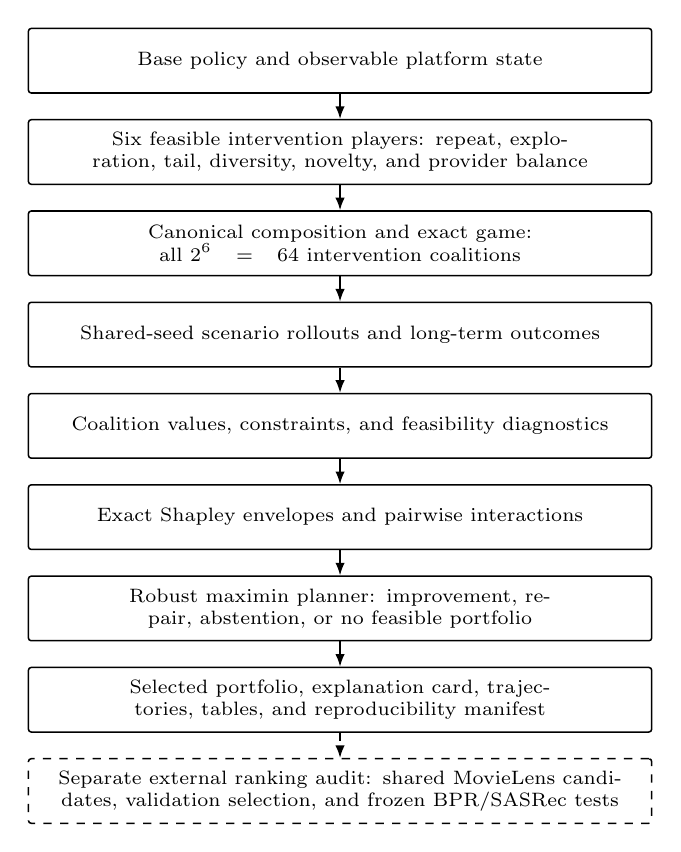
\begin{tikzpicture}[
  font=\scriptsize,
  node distance=3.2mm,
  stage/.style={draw=black, rounded corners=1pt, align=center, text width=0.64\textwidth, minimum height=8.2mm, inner sep=2.2pt, fill=white, line width=.55pt},
  audit/.style={stage, dashed},
  arrow/.style={-{Latex[length=1.6mm]}, draw=black, line width=.6pt}
]
\node[stage] (state) {Base policy and observable platform state};
\node[stage, below=of state] (players) {Six feasible intervention players: repeat, exploration, tail, diversity, novelty, and provider balance};
\node[stage, below=of players] (coalitions) {Canonical composition and exact game: all $2^6=64$ intervention coalitions};
\node[stage, below=of coalitions] (rollouts) {Shared-seed scenario rollouts and long-term outcomes};
\node[stage, below=of rollouts] (values) {Coalition values, constraints, and feasibility diagnostics};
\node[stage, below=of values] (credit) {Exact Shapley envelopes and pairwise interactions};
\node[stage, below=of credit] (planner) {Robust maximin planner: improvement, repair, abstention, or no feasible portfolio};
\node[stage, below=of planner] (output) {Selected portfolio, explanation card, trajectories, tables, and reproducibility manifest};
\node[audit, below=of output] (external) {Separate external ranking audit: shared MovieLens candidates, validation selection, and frozen BPR/SASRec tests};
\draw[arrow] (state) -- (players);
\draw[arrow] (players) -- (coalitions);
\draw[arrow] (coalitions) -- (rollouts);
\draw[arrow] (rollouts) -- (values);
\draw[arrow] (values) -- (credit);
\draw[arrow] (credit) -- (planner);
\draw[arrow] (planner) -- (output);
\draw[arrow, dashed] (output) -- (external);
\end{tikzpicture}
\caption{Vertical workflow of the proposed \CURE{} framework. The solid path defines, evaluates, attributes, and selects an intervention portfolio. The dashed final box is a separate external ranking audit and is not used to infer causal policy effects from MovieLens.}
\label{fig:workflow}
\end{figure}

\subsection{Exact coalition evaluation and common random numbers}

For a fixed seed and scenario, all coalitions are initialized from the same environment state and use the same event-indexed random-number construction. This common-random-number design aligns stochastic shocks across coalition evaluations and \emph{can} reduce the variance of paired differences when coalition outcomes are positively correlated under shared randomness; an observed difference is then attributable to the policy transformation rather than to a different synthetic cohort draw. Such variance reduction is not guaranteed. Accordingly, we evaluate its effect separately in Section~\ref{sec:robustness-extensions}: in the predeclared stochastic click-feedback variant, the observed variance ratios were approximately one, indicating no material variance reduction in that diagnostic. Seeds are independent across repetitions, and each run writes a manifest, JSONL events, coalition values, attribution envelopes, interaction diagnostics, decision data, trajectories, and generated tables and figures.

A coalition can still reduce utility, violate relevance, or fail a provider constraint; the grand coalition is in fact harmful in the observed behavioural scenarios. The common-random-number design merely ensures that a comparison between two coalitions is not dominated by an avoidable difference in simulated initial state. We preserve independent seeds because a common-random-number result from one seed is not a stability claim.

Every exact run has three audit layers. The game layer checks that all 64 masks are present for every scenario and that the Shapley efficiency gap is numerically zero. The planner layer records why a coalition is rejected, whether the base is feasible, and whether the final status is improvement, repair, abstention, or no feasible portfolio. The reporting layer materializes numbered tables and figures plus an asset registry. This makes the reported result traceable from a manuscript number to a seed, a configuration hash, and the underlying coalition rows.

The computational cost is transparent. With six players and four behavioural scenarios, one seed requires $64\times4=256$ rollouts. The primary behavioural stability study has 20 seeds, or 5,120 scenario--coalition rollouts. The one-at-a-time robustness study evaluates 15 configurations across five seeds; the joint Latin-hypercube study evaluates a baseline plus 24 joint configurations across five seeds. These are substantial but finite computations, and all completed summaries and checksums are retained in the reproducibility snapshot.

\subsection{Attribution, interactions, and direct selection}

The Shapley allocation obeys efficiency within every scenario; since $\Delta\Utility_m(\varnothing)=0$ by definition,
\begin{equation}
 \sum_{i\in\Players}\Shap_i^m=\Delta\Utility_m(\Players).
\label{eq:efficiency}
\end{equation}
This identity is a diagnostic: it is checked to machine precision in every exact game. Pairwise interactions are computed exactly under the declared Grabisch--Roubens convention. Positive interactions identify complementarity, whereas negative interactions identify combinations whose joint effect is lower than their separate effects imply.

Selection does not add Shapley values. Let $\mathcal{F}=\{S\subseteq\Players:\mathbf{1}_{\mathcal F}(S)=1\}$ be the feasible coalitions and let $\mathcal F_+=\mathcal F\setminus\{\varnothing\}$ be the feasible nonempty intervention coalitions. Coalitions are ordered first by decreasing $\underline\Delta(S)$ and, among equal values, by increasing cost, increasing cardinality, and canonical mask. The decision rule is casewise:
\begin{equation}
 (S^\star,\mathrm{status})=
 \begin{cases}
 \left(\arg\max_{S\in\mathcal F}\underline\Delta(S),\ \textsc{improvement}\right)
   & \begin{aligned}[t]&\text{if }\varnothing\in\mathcal F\text{ and}\\[-2pt]
     &\max_{S\in\mathcal F}\underline\Delta(S)>0,\end{aligned}\\[4pt]
 \left(\varnothing,\ \textsc{abstain}\right)
   & \begin{aligned}[t]&\text{if }\varnothing\in\mathcal F\text{ and}\\[-2pt]
     &\max_{S\in\mathcal F}\underline\Delta(S)\leq0,\end{aligned}\\[4pt]
 \left(\arg\max_{S\in\mathcal F_+}\underline\Delta(S),\ \textsc{repair}\right)
   & \begin{aligned}[t]&\text{if }\varnothing\notin\mathcal F\text{ and}\\[-2pt]
     &\mathcal F_+\neq\emptyset,\end{aligned}\\[4pt]
 \left(\varnothing,\ \textsc{no-feasible-portfolio}\right)
   & \begin{aligned}[t]&\text{if }\varnothing\notin\mathcal F\text{ and}\\[-2pt]
     &\mathcal F_+=\emptyset.\end{aligned}
 \end{cases}
\label{eq:improve}
\end{equation}
In improvement mode the base policy is feasible, so abstention preserves feasibility; in repair mode the base policy violates a constraint and $\varnothing$ is removed from the choice set, so the same maximin criterion chooses the least-worst feasible repair even when its numerical improvement is negative, or certifies that no feasible portfolio exists. This direct objective preserves the meaning of the outcome: Shapley values are explanatory credit; the selected policy is a constrained action.

\begin{center}
\fbox{\begin{minipage}{0.92\linewidth}
\textbf{Conditional guarantees and boundaries.}\vspace{2pt}

\scriptsize
\begin{tabularx}{\linewidth}{@{}>{\raggedright\arraybackslash}p{0.46\linewidth}>{\raggedright\arraybackslash}X@{}}
\textbf{Guaranteed for the evaluated table} & \textbf{Not guaranteed}\\
Full coalition enumeration; attribution without subset-sampling error; maximin feasible selection under the declared mode; and preference for a feasible repair over an infeasible base. & Scenario completeness; unseen-seed feasibility; real-world causal validity; or large-library tractability.\\
\end{tabularx}
\end{minipage}}
\end{center}

The explanation card reports both objects. For every selected intervention it records the robust-game Shapley value and the scenario-wise envelope. For an additional diagnostic it reports the \emph{budget-feasible marginal diagnostic}, defined as the unweighted mean of $\Delta\Utility_m(S\cup\{i\})-\Delta\Utility_m(S)$ over predecessor coalitions for which both $S$ and $S\cup\{i\}$ satisfy the budget constraint. If a player has no budget-feasible predecessor, the diagnostic is undefined and is reported as missing rather than silently set to zero. This quantity is not an axiomatic Shapley value and is not used for selection; it is retained only to expose marginal effects among operationally budget-deployable predecessors. The card header records the selected coalition and its robust lower improvement. This design prevents a familiar but misleading presentation in which a bar chart of attributions is treated as if it were itself an optimization result. A player can have a positive global contribution but not appear in the chosen coalition because it is redundant, consumes scarce injection capacity, violates a constraint in combination, or is dominated by a lower-cost feasible substitute.

The interaction table provides a complementary diagnostic. Let $I_{ij}^m$ denote the declared pairwise interaction of players $i$ and $j$ in scenario $m$. We compute the exact Shapley interaction index
\begin{equation}
 \begin{aligned}
 I_{ij}^m
 &=\sum_{S\subseteq\Players\setminus\{i,j\}}
 \frac{|S|!(|\Players|-|S|-2)!}{(|\Players|-1)!}\\[-2pt]
 &\quad\times\bigl[\Delta\Utility_m(S\cup\{i,j\})-\Delta\Utility_m(S\cup\{i\})\\
 &\hspace{56mm}-\Delta\Utility_m(S\cup\{j\})+\Delta\Utility_m(S)\bigr].
 \end{aligned}
\label{eq:interaction}
\end{equation}
Positive $I_{ij}^m$ means that the joint marginal contribution exceeds the additive baseline under the index; negative interaction means that combining them reduces their expected joint contribution. In the current framework, negative interactions are particularly informative because they often arise from an explicit operational mechanism: slot competition, overlap between long-tail and novelty proposals, or a reranking trade-off. The paper reports interactions as explanatory evidence and does not use a pairwise approximation to replace the exact portfolio search.

The reported $I_{ij}^m$ values are scenario-specific diagnostics. Unlike $\phi_i^{\mathrm{rob}}$, they are not presented as interactions of the maximin game $v^{\mathrm{rob}}$; computing the same index after substituting $v^{\mathrm{rob}}$ for $\Delta\Utility_m$ would define a separate robust-game interaction object. This distinction avoids implying that scenario-specific interaction signs automatically explain the nonlinear scenario minimum.

\begin{proposition}[Exact credit conservation]\label{prop:efficiency}
For every scenario $m$, the exact allocation in Eq.~\eqref{eq:shapley} satisfies Eq.~\eqref{eq:efficiency}. Thus all credited intervention value equals the full-coalition improvement over the base coalition in that scenario.
\end{proposition}

\begin{proposition}[Coalition well-definedness]\label{prop:well-defined}
Assume that candidate eligibility, score normalization, injection assignment, canonical transformation order, and tie breaking are deterministic conditional on the environment state and random seed. Then every coalition $S\subseteq\Players$ defines one policy transformation $\Policy_S$, independently of the permutation used to compute its Shapley marginal contribution.
\end{proposition}

\begin{proposition}[Repair feasibility ordering]\label{prop:repair}
If the base coalition is infeasible and $\mathcal F_+\neq\emptyset$, the repair rule returns a coalition $S^\star\in\mathcal F_+$ satisfying $\underline\Delta(S^\star)\geq\underline\Delta(S)$ for every $S\in\mathcal F_+$. It therefore never returns the infeasible base coalition.
\end{proposition}

\begin{proposition}[Decision admissibility]\label{prop:admissibility}
Conditional on the evaluated coalition table, Eq.~\eqref{eq:improve} returns the maximin feasible improvement when the base is feasible and a positive improvement exists; retains the feasible base otherwise; returns the maximin feasible repair when the base is infeasible and $\mathcal F_+\neq\emptyset$; and reports \textsc{no-feasible-portfolio} when no feasible repair exists.
\end{proposition}

The propositions do not claim that the finite scenario set is the true real-world environment. They establish properties conditional on the game and constraint definitions, which is the appropriate theoretical level for a decision layer. Proofs are included in Appendix~\ref{app:proofs}.

\subsection{Algorithms and complexity}
The complete evaluation and planner pseudocode, together with rollout and memory cost accounting, is provided in Appendix~\ref{app:proofs}. In brief, coalition evaluation costs $O(M2^nC_{\mathrm{roll}})$, and exact Shapley and pairwise interaction computation cost $O(Mn2^n)$ and $O(Mn^2 2^n)$ after coalition values are available. The full six-player, four-scenario configuration evaluates $64\times4=256$ rollouts per seed. This exponential dependence is why the paper treats exact enumeration as an auditable benchmark for a bounded intervention library rather than a solution for hundreds of interventions.

\subsection{Controlled oracle regimes}

Before behavioural simulation, nine analytic regimes verify the mechanics of the game and planner: additive, complementary, redundant, antagonistic, short delayed-fatigue, long delayed-fatigue, two provider-repair regimes, and misspecified ambiguity. In well-specified regimes, estimated and oracle games agree by construction. The misspecified regime is intentionally different: the estimated game selects repeat cap while the oracle game selects exploration. It tests whether the framework falsely treats self-consistency as causal recovery. The misspecification diagnostics are: oracle regret, the robust lower improvement lost by deploying the estimated selection instead of the oracle selection; Shapley mean absolute error and sign accuracy between estimated and oracle scenario attributions; and point coverage, the fraction of players whose oracle Shapley value falls inside the estimated scenario Shapley envelope $[\underline{\Shap}_i,\overline{\Shap}_i]$ of Eq.~\eqref{eq:region}.



\subsection{Behavioural robustness designs}

The behavioural benchmark has four scenarios: nominal, fatigue stress, popularity stress, and mixed stress. The full configuration uses 120 users, 240 items, 18 providers, 10 categories, a 12-step horizon, and a slate of 10. Every numerical scenario parameter---fatigue multipliers $\alpha_m$, popularity-feedback multipliers $\beta_m$, and satisfaction shifts $\delta_m$---is listed in Table~\ref{tab:scenarios} of Appendix~\ref{app:protocol}; nothing about the scenarios is tuned after observing outcomes. The one-at-a-time study changes fatigue strength, repeat threshold, horizon, provider threshold, provider-balance strength, delayed novelty preference drift, and exploration cost. The joint Latin-hypercube design samples these assumptions jointly \cite{mckay1979latin}. Neither study selects a favourable configuration; all configurations and all seed-level decisions are retained. In these designs the environment assumptions vary while the decision-maker's utility weights $(w_s,w_r,w_f,w_c)$ stay fixed; the complementary sensitivity question---varying the objective itself---is studied separately in Section~\ref{sec:objective-sensitivity}. Figures~\ref{fig:lhs} and~\ref{fig:oat} summarize the full-game attribution and selected OAT effects, respectively.

\begin{figure}[t]
\centering
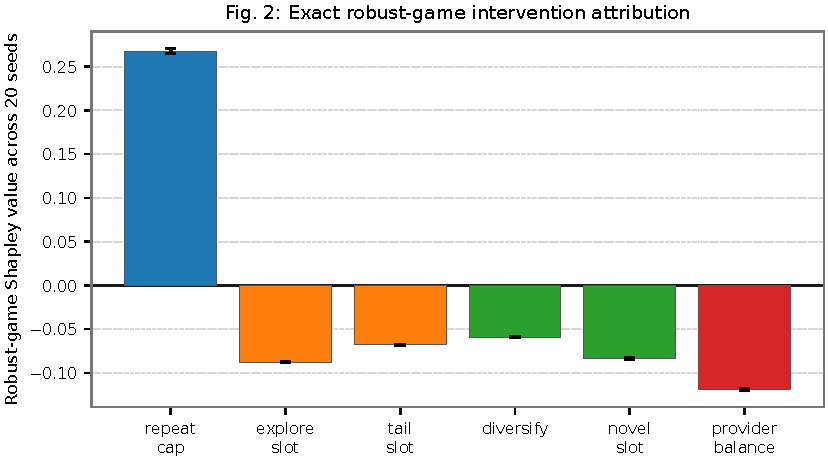
\includegraphics[width=\linewidth]{figures/figure_02_exact_attribution.pdf}
\caption{Exact robust-game Shapley values for the maximin characteristic function across the 20 independent full behavioural seeds. Error bars are seed-level sample standard deviations. This figure is the additive attribution of the actual planner objective, not a scenario-envelope summary.}
\label{fig:lhs}
\end{figure}

\begin{figure}[t]
\centering
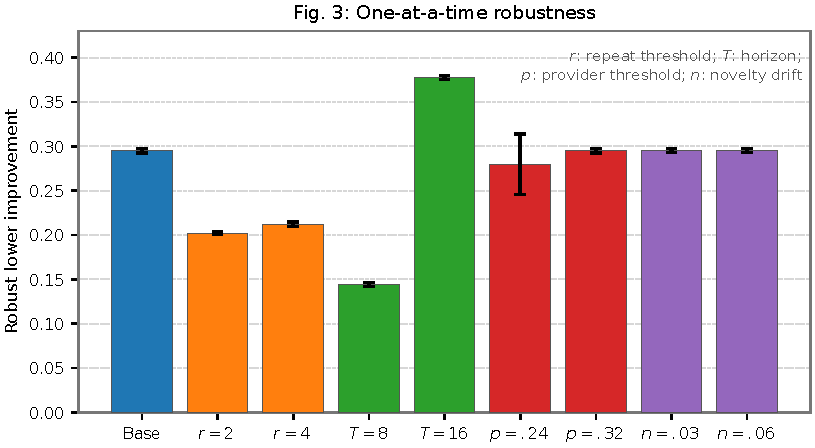
\includegraphics[width=\linewidth]{figures/figure_03_oat_sensitivity.pdf}
\caption{Selected one-at-a-time sensitivity results for mean robust lower improvement: horizon, repeat threshold, provider threshold, and novelty drift are shown; fatigue strength, provider-balance strength, and exploration cost additionally appear in Table~\ref{tab:oat}. Error bars are sample standard deviations over five independent seeds.}
\label{fig:oat}
\end{figure}





\subsection{External ranking protocol}\label{sec:external-protocol}

MovieLens-1M is used only to test recommender implementation robustness. The dataset contains 6,040 users, 3,706 items, and 1,000,209 ratings \cite{harper2015movielens}. A \emph{positive interaction} is a rating of at least four stars ($\mathrm{rating}\geq4$); this threshold is fixed before modelling and yields 575,281 positives. No user-level filtering is applied beyond the split rule below. We construct a chronological leave-one-out split from positive interactions: interactions are sorted per user by timestamp (ties by item identifier), users with fewer than three positives are excluded from evaluation, the last positive of each remaining user is the test target, the previous one is the validation target, and all earlier positives form training. Evaluation then proceeds in ascending user-identifier order over the first 1,000 warm-target users; we report on these 1,000 users, together with one cold test target, rather than silently dropping the cold case or reweighting the evaluation. For every evaluated user, all models receive the identical candidate set
\begin{equation}
 \mathcal{C}_u=\mathcal{I}_{\mathrm{train}}\setminus\mathcal{I}_{u,\mathrm{train}}.
\label{eq:candidates}
\end{equation}
A held-out target absent from the training catalogue is counted as cold rather than silently removed. The final evaluations report 1,000 warm-target users, one cold test target, mean candidate count 3,436.958, and candidate counts from 2,739 to 3,521. For a warm target $i_u^+$ with rank $q_u$ in the ordered candidate list, the per-user metrics are
\begin{equation}
 \mathrm{Recall@}k(u)=\mathbf{1}\{q_u\leq k\},\qquad
 \mathrm{NDCG@}k(u)=\frac{\mathbf{1}\{q_u\leq k\}}{\log_2(q_u+1)},
\label{eq:ranking-metrics}
\end{equation}
and reported values are means over warm evaluated users with cold-target coverage stated separately. Score ties are broken deterministically by ascending item identifier before ranking. Because every evaluated user has exactly one binary held-out target, $\Recall$ coincides identically with Hit Rate at the same $k$; we report the quantity as $\Recall$ in the MovieLens-1M tables and as ``Hit Rate'' in the MovieLens-25M diagnostic, but the two are the same statistic under this protocol. With a single relevant item, $\NDCG$ uses the standard single-target ideal discount \cite{jarvelin2002cumulated}. This definition makes the candidate protocol part of the estimand rather than an implementation detail.

The protocol has three gates. First, hyperparameters are selected by validation $\NDCG$ only. Second, the frozen selected configuration is trained once for the final audit and its best validation checkpoint is restored before test ranking. Third, the configuration is replicated over fixed independent seeds without retuning. The evaluator asserts zero seen-item leakage, zero missing-target violations, identical candidates for all compared models, and descending-score correctness. This protocol guards against metric improvements produced by an evaluator difference rather than by a recommender.

The popularity baseline is fit on training interactions only. BPR-MF \cite{rendle2009bpr} and SASRec \cite{kang2018sasrec} are trained with pairwise ranking losses, selected solely by validation $\NDCG$, restored at their best validation checkpoints, and replicated under frozen configurations without test-driven retuning. Model losses, negative sampling, selected hyperparameters, and complete search budgets are reported in Appendix~\ref{app:audit}.

The audit also records pairwise training and validation accuracy. These quantities are not used as ranking metrics or selection targets; they are sanity checks that a personalized model has learned a directional preference signal without candidate leakage. For the final SASRec audit, the popularity and SASRec models both have zero critical audit violations and the SASRec best validation epoch equals the restored checkpoint epoch (20). The same audit is rerun within every fixed-configuration replication.

The user-level estimand averages each evaluated user's outcome over the five frozen optimizer seeds before forming the paired model-minus-popularity difference $d_u$. We report the paired bootstrap interval for $\overline d$ and $d_z=\overline d/s_d$, where $s_d$ is the sample standard deviation of the user differences. Binary seed-42 Hit@10 is tested by exact McNemar; five-seed averaged Hit@10 is no longer binary and is tested by a paired sign test; five-seed averaged NDCG uses a paired sign-flip permutation test. Users are the inferential units for this fixed benchmark cohort, not independent draws that justify unrestricted generalization to arbitrary deployment populations.

\subsection{Implementation and reproducibility}

The artifact is implemented in Python with typed configuration, deterministic seeds, JSONL events, CSV tables, and a checksumed snapshot. Exact intervention games use CPU-first NumPy simulation. External BPR and SASRec use PyTorch with Apple Silicon MPS when available; BPR uses Adam, item bias, and mixed negatives, while SASRec uses causal self-attention, right-padded sequences, and validation checkpointing. The final snapshot stores source manifests, final configurations, audit tables, loss and validation histories, seed metrics, paired metrics, calibration summaries, controlled-regime assets, and SHA-256 checksums. The code and the manuscript assets are available with the project repository.

\section{Experimental results}\label{sec:results}

\subsection{Research questions and evidence levels}

The results follow six questions. \textbf{RQ1}: does the exact game recover known additive, interaction, delay, repair, and misspecification structures? \textbf{RQ2}: what does the planner select in the primary behavioural configuration, and is that decision stable across seeds? \textbf{RQ3}: when selectors disagree, do repair semantics or portfolio search change the admissible decision? \textbf{RQ4}: how does the decision change under isolated and joint calibration stress? \textbf{RQ5}: do audited BPR and SASRec implementations improve chronological ranking over popularity under identical candidates? \textbf{RQ6}: how sensitive is the decision to the declared utility weights and constraint vector? Supporting approximation, scalability, and learned-base-policy diagnostics appear in Appendix~\ref{app:additional-diagnostics}.

RQ1--RQ4 and RQ6 concern the disclosed \Sim{} environment. RQ5 is a separate external ranking audit on MovieLens-1M; it neither identifies a long-run intervention effect nor validates the portfolio-selection layer.

\subsection{RQ1: controlled recovery and misspecification}\label{sec:rq1}

Table~\ref{tab:regimes} reports the controlled-regime result. The estimated game reproduces the specified estimated selection in all nine regimes. Oracle selection agrees in eight. The exception is deliberately misspecified: the estimated game selects \texttt{repeat\_cap}, while the oracle selects \texttt{explore\_slot}. Estimated recovery is therefore not treated as proof of oracle recovery. The misspecified setting has oracle regret $0.19$, Shapley mean absolute error $0.06$, sign accuracy $0.667$, and point coverage $0.667$.

\begin{table*}[t]
\caption{Controlled oracle-regime validation. ``Estimated match'' compares the selected estimated-game portfolio with the declared estimated target; ``oracle match'' compares it with the true-game portfolio.}\label{tab:regimes}
\centering
\scriptsize
\setlength{\tabcolsep}{3pt}
\resizebox{\textwidth}{!}{%
\begin{tabular}{@{}llccc@{}}
\toprule
Regime & Estimated selected portfolio & Oracle selected portfolio & Estimated match & Oracle match / regret\\
\midrule
Additive & repeat cap + exploration + tail + provider balance & repeat cap + exploration + tail + provider balance & yes & yes / 0.00\\
Complementary & repeat cap + exploration & repeat cap + exploration & yes & yes / 0.00\\
Redundant & tail slot & tail slot & yes & yes / 0.00\\
Antagonistic & exploration slot & exploration slot & yes & yes / 0.00\\
Delayed fatigue, short horizon & abstain & abstain & yes & yes / 0.00\\
Delayed fatigue, long horizon & repeat cap & repeat cap & yes & yes / 0.00\\
Provider repair, balancing & provider balance & provider balance & yes & yes / 0.00\\
Provider repair, repeat & repeat cap & repeat cap & yes & yes / 0.00\\
Misspecified ambiguity & repeat cap & exploration slot & yes & no / 0.19\\
\bottomrule
\end{tabular}}
\end{table*}

Table~\ref{tab:interaction-diagnostics} makes the interaction evidence explicit. It reports the sign recovered from the exact scenario-specific interaction tables in the three analytic non-additive regimes. These are mechanism checks rather than estimates from the behavioural benchmark: complementarity raises the joint marginal contribution, whereas redundancy and antagonism lower it.

\begin{table}[t]
\caption{Interaction diagnostics in the analytic regimes. Signs are those of the exact scenario-specific Grabisch--Roubens interaction index.}\label{tab:interaction-diagnostics}
\centering
\scriptsize
\setlength{\tabcolsep}{4pt}
\begin{tabularx}{\linewidth}{@{}lXcl@{}}
\toprule
Regime & Intervention pair & Sign & Decision implication\\
\midrule
Complementary & repeat cap + exploration & positive & select jointly\\
Redundant & tail slot + novelty slot & negative & retain one under tie/cost rule\\
Antagonistic & exploration + diversity & negative & avoid the harmful pair\\
\bottomrule
\end{tabularx}
\end{table}

This result provides a needed negative control. A cooperative attribution layer can be internally consistent and still be wrong when its model of the environment is wrong. The paper therefore reports estimated and oracle recovery separately rather than compressing them into one success rate.

The remaining regimes test the distinction between contribution and decision. In the complementary regime, repeat cap and exploration are weak alone but selected jointly. In the redundant regime, tail and novelty overlap and the planner selects one player under its deterministic cost and tie rule. In the antagonistic regime, exploration and diversity are individually useful but jointly harmful, so the selected policy avoids the pair. The two provider-repair regimes start from an infeasible base and select different repairs: provider balancing in one and repeat suppression in the other. These cases show why a framework that independently ranks interventions cannot substitute for a coalition search with explicit repair semantics.

The short- and long-horizon delayed-fatigue regimes additionally test temporal interpretation. With the short horizon, the base is feasible and the planner abstains because repeat suppression has not yet recovered its immediate cost. With the longer horizon, repeat cap is selected. The switch is not a change in implementation or attribution convention; it is a change in the declared decision horizon. This is the minimal controlled demonstration that a myopic metric and a long-horizon intervention decision need not agree.

\subsection{RQ2: behavioural selection over independent seeds}\label{sec:rq2}

The full behavioural study evaluates all 64 coalitions under four scenarios across 20 independent seeds. Repeat cap is selected in 20/20 seeds. The mean robust lower improvement is $0.29371$ with standard deviation $0.00258$ and range $[0.28928,0.29709]$ (CURE-Sim normalized utility units). Fourteen of 20 decisions are repairs because the base violates the provider-disparity constraint; six are improvements from a feasible base. The selected portfolio is feasible in every seed. Table~\ref{tab:behavioural} summarizes the three seed studies.

The independent five-seed full run provides a second check: repeat cap is selected in 5/5 seeds, with mean lower improvement $0.29488$ and standard deviation $0.00244$. The quick configuration is not used for the primary behavioural claim: it selects repeat cap in four seeds and repeat cap plus tail slot in one, with one negative-improvement repair. It is retained only as an implementation and runtime check.

\begin{table*}[t]
\caption{Behavioural exact-game seed studies. Lower improvement is the worst-scenario utility change relative to the base policy.}\label{tab:behavioural}
\centering
\scriptsize
\setlength{\tabcolsep}{3pt}
\resizebox{\textwidth}{!}{%
\begin{tabular}{@{}lrrrrl@{}}
\toprule
Study & Seeds & Repeat-cap selection & Lower improvement & SD & Planner modes\\
\midrule
Quick five-seed & 5 & 4/5 & 0.01241 & 0.03908 & 4 improve, 1 repair\\
Full five-seed & 5 & 5/5 & 0.29488 & 0.00244 & 1 improve, 4 repair\\
Full twenty-seed & 20 & 20/20 & 0.29371 & 0.00258 & 6 improve, 14 repair\\
\bottomrule
\end{tabular}}
\end{table*}

The grand coalition is budget-infeasible in every seed of the full configuration ($c(\Players)=0.49>B=0.35$), and its raw robust-game value is negative: for example, $\underline{\Delta}(\Players)=-0.14430$ at seed 42 (CURE-Sim normalized utility units), computed directly from the scenario-indexed coalition values. Table~\ref{tab:selector-baselines} reports this raw value separately from the zero fallback payoff of the grand-coalition \emph{selector}, which deploys the full coalition only when it is feasible. The grand coalition is retained only as a diagnostic, not as a selectable portfolio. This rejects an additive ``more interventions is always better'' interpretation. Interaction analysis explains why: several injection and reranking combinations introduce relevance, cost, or fatigue trade-offs that a single-intervention ablation cannot expose.

\begin{table*}[t]
\caption{Held-out selector evaluation. Portfolios are selected on five seeds and evaluated on 20 disjoint seeds. The independent inferential unit is the evaluation seed; 100 cross-product rows are retained for traceability but are not treated as 100 independent observations.}\label{tab:selector-baselines}
\centering
\scriptsize
\setlength{\tabcolsep}{3pt}
\resizebox{\textwidth}{!}{%
\begin{tabular}{@{}lrrrl@{}}
\toprule
Selector & Held-out robust lower improvement & SD & Difference versus CURE & Exact sign-test $p$\\
\midrule
CURE exact maximin & 0.294584 & 0.002031 & --- & ---\\
Best singleton & 0.294584 & 0.002031 & 0.000000 & 1.000000\\
Robust Shapley-1 & 0.294584 & 0.002031 & 0.000000 & 1.000000\\
Robust Shapley-budget & 0.294584 & 0.002031 & 0.000000 & 1.000000\\
Greedy robust & 0.294584 & 0.002031 & 0.000000 & 1.000000\\
Nominal-scenario selector & 0.294584 & 0.002031 & 0.000000 & 1.000000\\
Random feasible & 0.059153 & 0.112314 & -0.235431 & 0.000002\\
Grand-coalition diagnostic\footnotemark[1] & 0.000000 & 0.000000 & -0.294584 & 0.000002\\
\bottomrule
\end{tabular}}
\footnotetext[1]{$0$ denotes the selector's fallback payoff from retaining the base when the grand coalition is infeasible; it is not the grand coalition's raw game value, which is negative (Section~\ref{sec:rq2}).}
\end{table*}

The primary configuration is intentionally not evidence of superiority over simpler selectors: exact CURE, singleton, Shapley-ranked, greedy, and nominal selectors all converge to repeat cap. It instead shows that the fully enumerated method does not manufacture a more complex portfolio when one intervention is dominant. Random feasible selection performs worse, and the grand coalition is a budget-infeasible diagnostic rather than a candidate action.

The decision modes are as informative as the selected player. In the full twenty-seed study, the base is infeasible in 14 seeds, principally because provider disparity crosses the declared upper bound. Those outputs are repairs, not failed improvements. Repeat suppression can repair provider disparity indirectly because repeatedly exposed, high-popularity items also concentrate exposure on their providers; demoting those items releases slate positions to a broader provider set while reducing fatigue. At seed 42, for example, the selected repeat-cap policy has upper provider disparity $0.225872$, below the declared $0.28$ threshold. In the remaining six seeds, the base is feasible and repeat cap is selected as an improvement.

The result also illustrates why the full coalition is not a useful default. A system might reason that enabling all safeguards is conservative. Here, the grand coalition is repeatedly harmful because three slot interventions compete for capacity, rerankers can reduce relevance, and total cost can exceed the budget. Exact enumeration makes this failure visible without assuming pairwise additivity. In a larger intervention library, screening or approximation would be required; the present six-player study provides a clean benchmark in which the portfolio optimum is known exactly.

The primary game's robust Shapley allocation is likewise dominated by repeat cap (Fig.~\ref{fig:lhs}). We do not use that dominance as evidence that exact interaction reasoning is necessary in every instance. The controlled complementary and antagonistic regimes, together with the disagreement cases below, provide the settings in which portfolio structure and repair semantics change the decision.

\subsection{RQ3: when portfolio reasoning changes the decision}\label{sec:divergent-selectors}

The tied primary comparison motivates a targeted diagnostic. A screening rule was fixed before inspecting screening outcomes: among archived LHS points whose five-seed decisions were not uniformly repeat cap, configurations were examined in declared design order using seed 42, and the first points at which at least two substantive selectors chose different masks were retained. Thus, the configurations were \emph{selected by a predeclared disagreement-screening rule}; the configurations themselves were not individually predeclared as favourable cases.

The retained points expose different failures (Table~\ref{tab:divergent-diagnostics}). In \texttt{lhs-012}, the base is infeasible and every feasible repair has negative improvement relative to that infeasible base. Budgeted-Shapley and greedy marginal rules therefore stop at $\varnothing$, which is not an admissible repair. This is a \emph{repair-semantics failure}. In \texttt{lhs-009}, repeat cap alone has positive value but violates the disparity constraint, while the only feasible singleton has negative value; the best feasible repair is repeat cap plus tail slot. This is a \emph{portfolio-search failure}. The two points are retained because they isolate distinct decision failures, not because they maximize a numerical advantage for \CURE{}.

\begin{table*}[t]
\caption{Two configurations selected by the disagreement-screening rule (seed 42). The cases isolate repair-semantics and portfolio-search failures.}\label{tab:divergent-diagnostics}
\centering
\scriptsize
\setlength{\tabcolsep}{4pt}
\begin{tabularx}{\textwidth}{@{}p{0.10\textwidth}p{0.19\textwidth}X X X@{}}
\toprule
Case & Diagnostic & Exact constrained planner & Feasible singleton / nominal selector & Budgeted-Shapley / greedy\\
\midrule
\texttt{lhs-012} & Repair semantics & provider balance (feasible repair) & provider balance; nominal ties the planner & $\varnothing$; retains infeasible base\\
\texttt{lhs-009} & Portfolio search & repeat cap + tail slot; $+0.192848$, feasible & provider balance; $-0.118509$, feasible; nominal ties the planner & $\varnothing$; retains infeasible base\\
\bottomrule
\end{tabularx}
\end{table*}

The held-out protocol freezes each selector's choices on seeds 42--46 and evaluates them on seeds 200--219. Table~\ref{tab:divergent-heldout-summary} separates raw utility from admissibility: a raw value of $0$ for $\varnothing$ is not treated as numerically superior when the base is infeasible. In \texttt{lhs-012}, the exact planner improves on the feasible singleton and Shapley-1 rules in all 20 evaluation seeds but ties the nominal-scenario selector. In \texttt{lhs-009}, the exact planner again ties the nominal selector and outperforms the singleton-based rules because they cannot recover the positive-valued two-intervention repair.

\begin{table*}[t]
\caption{Held-out summary for the disagreement cases. Raw lower improvement is reported even for infeasible frozen outputs; admissible differences are reported only when the compared decision is feasible. Feasibility rates are archived out-of-sample diagnostics, not guarantees of the selection problem.}\label{tab:divergent-heldout-summary}
\centering
\scriptsize
\setlength{\tabcolsep}{2pt}
\begin{tabular}{@{}p{0.09\textwidth}>{\raggedright\arraybackslash}p{0.315\textwidth}>{\raggedleft\arraybackslash}p{0.15\textwidth}>{\raggedleft\arraybackslash}p{0.10\textwidth}>{\raggedleft\arraybackslash}p{0.18\textwidth}@{}}
\toprule
Case & Selector & Raw lower improvement & Feasible rate & Admissible difference vs. CURE\\
\midrule
\multirow{4}{*}{\texttt{lhs-012}} & CURE exact maximin & $-0.089270$ & 0.70 & ---\\
 & Best singleton / robust Shapley-1 & $-0.100579$ & 0.70 & $-0.011309$\\
 & Nominal-scenario selector & $-0.089270$ & 0.70 & $0.000000$\\
 & Budgeted-Shapley / greedy ($\varnothing$) & $0.000000$ & 0.10 & NA\\
\midrule
\multirow{4}{*}{\texttt{lhs-009}} & CURE exact maximin & $+0.198583$ & 0.47 & ---\\
 & Best singleton / robust Shapley-1 & $-0.039305$ & 0.82 & $-0.237888$\\
 & Nominal-scenario selector & $+0.198583$ & 0.47 & $0.000000$\\
 & Budgeted-Shapley / greedy & $+0.052876$ & 0.02 & NA\\
\bottomrule
\end{tabular}
\end{table*}

Robustness in Eq.~\eqref{eq:robust-feasibility} is over the declared scenario set conditional on the selection seed $\zeta$; it is not a chance constraint over simulator initializations. Consequently, held-out feasibility rates of $0.70$ and $0.47$ are out-of-sample diagnostics rather than contradictions of the optimization guarantee. A generalized deployment rule could additionally require
\begin{equation}
 \Pr_{\zeta}\!\left[\mathbf 1_{\mathcal F}(S;\zeta)=1\right]\geq 1-\alpha,
\label{eq:chance-feasibility}
\end{equation}
or enforce feasibility across all calibration seeds. This extension would trade utility against initialization-level reliability and is not evaluated in the present artifact.

\subsection{RQ4: calibration robustness and portfolio switches}\label{sec:rq3}

The one-at-a-time study contains 15 predeclared configurations and five seeds per configuration. Repeat cap appears in every selected portfolio (75/75 seed decisions); it is the exact portfolio in 74/75 decisions. The exception occurs at the strict provider threshold 0.24, where one seed selects repeat cap plus tail slot. The result is stable but not invariant in magnitude. Shortening the horizon from 12 to 8 reduces mean lower improvement from $0.29488$ to $0.14397$; extending it to 16 increases it to $0.37785$. Altering the repeat threshold to 2 or 4 changes the mean to $0.20206$ and $0.21226$, respectively. These are expected behavioural sensitivities, not a failure of the framework.

\begin{table*}[t]
\caption{Selected one-at-a-time calibration results. Every row has five independent seeds. The table reports actual archived summaries.}\label{tab:oat}
\centering
\scriptsize
\setlength{\tabcolsep}{3pt}
\resizebox{\textwidth}{!}{%
\begin{tabular}{@{}lrrrll@{}}
\toprule
Assumption & Value & Lower improvement mean & SD & Base-feasible rate & Modal portfolio\\
\midrule
Baseline & --- & 0.29488 & 0.00244 & 0.20 & repeat cap\\
Fatigue strength & 0.75 & 0.29488 & 0.00244 & 0.20 & repeat cap\\
Fatigue strength & 1.25 & 0.29488 & 0.00244 & 0.20 & repeat cap\\
Repeat threshold & 2 & 0.20206 & 0.00175 & 0.20 & repeat cap\\
Repeat threshold & 4 & 0.21226 & 0.00240 & 0.20 & repeat cap\\
Horizon & 8 & 0.14397 & 0.00230 & 0.60 & repeat cap\\
Horizon & 16 & 0.37785 & 0.00220 & 0.20 & repeat cap\\
Provider threshold & 0.24 & 0.27997 & 0.03397 & 0.00 & repeat cap (modal frequency 4/5)\\
Provider threshold & 0.32 & 0.29488 & 0.00244 & 0.60 & repeat cap\\
Provider-balance strength & 0.15 & 0.29488 & 0.00244 & 0.20 & repeat cap\\
Provider-balance strength & 0.55 & 0.29488 & 0.00244 & 0.20 & repeat cap\\
Novelty drift & 0.03 & 0.29502 & 0.00249 & 0.20 & repeat cap\\
Novelty drift & 0.06 & 0.29513 & 0.00252 & 0.20 & repeat cap\\
Exploration cost & 0.05 & 0.29488 & 0.00244 & 0.20 & repeat cap\\
Exploration cost & 0.15 & 0.29488 & 0.00244 & 0.20 & repeat cap\\
\bottomrule
\end{tabular}}
\end{table*}

Several rows are identical to the baseline at the displayed precision. Provider-balance strength and exploration cost do not change the selected-policy summary because their corresponding interventions are absent from the selected coalition. The two fatigue-strength rows are also unchanged in the archived selected-policy summary; this invariance should not be read as evidence that every coalition value is unchanged or that the parameter is irrelevant. The archived coalition tables, rather than this selected-policy table alone, are the appropriate wiring diagnostic.

The Latin-hypercube study is the more stringent test because it changes assumptions jointly. It contains a baseline plus 24 configurations, five seeds each, for 125 decisions. Repeat cap appears in 114/125 selected portfolios, but the framework also selects provider balance, tail-enhanced portfolios, repeat cap plus exploration, and abstention. Across the 25 configuration-level modal portfolios, 18 are repeat cap alone, three are repeat cap plus tail slot, two are provider balance, one is repeat cap plus exploration, and one is abstention. Eighty-three of 125 decisions are repair-mode cases and 42 are improvement-mode cases; four of the improvement-mode cases end in abstention, so mode counts and final-status counts are distinct objects. The framework therefore does not mechanically choose the same player under joint extreme conditions; the documented switches follow changes in feasibility and scenario assumptions.

The LHS study changes the interpretation of the OAT finding. The OAT result supports local robustness: along each isolated axis in the declared range, repeat cap remains present in every selected portfolio. It does not prove global invariance under combined changes. The LHS result supplies the needed qualification. In several joint configurations the modal solution is provider balancing, and in another the modal choice is abstention. All switching cases are retained; they identify the boundary of the repeat-cap conclusion and show that the framework can express a feasibility-driven portfolio switch rather than merely amplifying the strongest average player.

For reporting, we treat the LHS configurations as a predeclared stress design rather than as an i.i.d. sample from a real distribution of platforms. The counts $114/125$ and $83/125$ are therefore descriptive frequencies over the design, not estimates of an unknown global deployment probability. The design-level attribution--inclusion plot is retained in Appendix~\ref{app:calibration}, where its aggregation caveat can be read beside the full portfolio distribution.

\subsection{RQ5: external ranking audit on MovieLens-1M}\label{sec:rq4}

The external evaluation is deliberately separated from the causal benchmark. Popularity, BPR-MF, and SASRec use the same chronological split and candidates. BPR is selected through staged validation search, then audited once and replicated over fixed seeds. SASRec is selected by validation $\NDCG$, audited once on the untouched test set, and replicated without retuning. The final audit has zero seen-item, missing-target, candidate-equality, and descending-score violations for every compared model.

Table~\ref{tab:external} reports the five-seed fixed-configuration summaries. Popularity has $\Recall=0.049$ and $\NDCG=0.02552$. BPR reaches $0.08800\pm0.00354$ recall and $0.04384\pm0.00167$ NDCG. SASRec reaches $0.14520\pm0.00311$ recall and $0.07424\pm0.00281$ NDCG. All SASRec seed-level gains over popularity are positive: recall gains range from $0.091$ to $0.099$ and NDCG gains from $0.04553$ to $0.05293$. These are reproducible ranking results under the protocol; they are not estimates of causal intervention benefit.

At the seed level, the paired differences against popularity are all positive for both models and both metrics (5/5 seeds). The exact two-sided sign test on five paired seeds has a minimum attainable $p$-value of $2(0.5)^5=0.0625$, which is not conventionally significant; a paired $t$-test on the five seed differences is significant ($|t(4)|\geq24.6$, $p\leq1.6\times10^{-5}$, $d_z\geq11.0$) but treats optimizer seeds as the inferential unit and assumes normality of seed effects.

The pre-specified user-level analysis retrains the frozen final configurations for seeds 42--46, exports one hit/NDCG row per evaluated warm user, and applies paired inference (Table~\ref{tab:ml1m-userlevel}). With the user as the inferential unit for this fixed cohort ($n=1{,}000$), every comparison is significant after Holm correction across the model$\times$metric family. At seed 42, exact McNemar tests on binary hit indicators give $p\leq1.5\times10^{-4}$, while seed-42 NDCG sign-flip tests give $p\leq0.0014$. For the five-seed per-user means, the averaged hit outcome is not binary: Table~\ref{tab:ml1m-userlevel} therefore uses a paired sign test for Hit@10 and a paired sign-flip permutation test for NDCG@10. All paired user-bootstrap confidence intervals for the mean differences exclude zero. Effect sizes are small-to-moderate ($d_z$ between $0.099$ and $0.280$), so the claim is a statistically supported improvement under the audited warm-item protocol, not a large-effect or deployment-population claim. These remain chronological-ranking results: they do not estimate causal policy effects and do not validate the \CURE{} portfolio-selection layer.

\begin{table*}[t]
\caption{MovieLens-1M user-level paired inference against popularity ($n=1{,}000$ warm users; five-seed per-user means). Confidence intervals use a paired user bootstrap. Holm-adjusted $p$-values use a paired sign test for Hit@10 and a paired sign-flip permutation test for NDCG@10.}\label{tab:ml1m-userlevel}
\centering
\scriptsize
\setlength{\tabcolsep}{3pt}
\resizebox{\textwidth}{!}{%
\begin{tabular}{@{}llrrrr@{}}
\toprule
Model & Metric & Mean difference & 95\% CI & $d_z$ & Holm $p$\\
\midrule
BPR-MF + bias & Hit@10 & $+0.039000$ & $[0.0206,0.0574]$ & 0.136 & $1.5\times10^{-10}$\\
BPR-MF + bias & NDCG@10 & $+0.018320$ & $[0.0080,0.0287]$ & 0.109 & $1.1\times10^{-11}$\\
SASRec & Hit@10 & $+0.096200$ & $[0.0752,0.1176]$ & 0.280 & $1.7\times10^{-40}$\\
SASRec & NDCG@10 & $+0.048716$ & $[0.0358,0.0617]$ & 0.241 & $7.5\times10^{-43}$\\
\bottomrule
\end{tabular}}
\end{table*}

\begin{table*}[t]
\caption{MovieLens-1M fixed-configuration five-seed ranking results under shared warm-item candidates. Mean $\pm$ sample standard deviation over optimizer seeds; popularity is deterministic for the fixed split. With one binary held-out target per user, $\Recall$ equals Hit Rate.}\label{tab:external}
\centering
\scriptsize
\setlength{\tabcolsep}{2pt}
\resizebox{\textwidth}{!}{%
\begin{tabular}{@{}lrrrr@{}}
\toprule
Model & $\Recall$ & $\NDCG$ & $\Delta\Recall$ vs. popularity & $\Delta\NDCG$ vs. popularity\\
\midrule
Popularity & 0.04900 & 0.02552 & --- & ---\\
BPR-MF + bias & $0.08800\pm0.00354$ & $0.04384\pm0.00167$ & $0.03900\pm0.00354$ & $0.01832\pm0.00167$\\
SASRec & $0.14520\pm0.00311$ & $0.07424\pm0.00281$ & $0.09620\pm0.00311$ & $0.04872\pm0.00281$\\
\bottomrule
\end{tabular}}
\end{table*}

\subsection{RQ6: objective and constraint sensitivity}\label{sec:rq5}

RQ6 varies the decision-maker's declared objective and feasible set while holding the archived coalition outcomes fixed. Approximation, common-random-number, scalability, and learned-base-policy diagnostics are retained in Appendix~\ref{app:additional-diagnostics} so that they do not interrupt the main decision argument.

\subsubsection{Objective sensitivity: utility weights and the constraint frontier}\label{sec:objective-sensitivity}

The environment studies above vary simulator assumptions while holding the decision-maker's objective fixed. The objective itself, however, is normative: the weights $(w_s,w_r,w_f,w_c)$ encode a platform's declared trade-offs, and the constraint vector $(B,r_{\min},d_{\max},f_{\max})$ encodes its operating limits. We therefore stress the decision with respect to both objects. The archived seed-42 exact game (asset \texttt{divergent\_selector\_holdout/screening/baseline}) stores the step-aggregated satisfaction, retention, fatigue, relevance, disparity, and cost of every coalition and scenario. Utility under any weight vector is therefore a linear recombination of stored outcomes, and feasibility under any constraint vector is a threshold test on stored margins; both sweeps are exact recombinations of the archived rollouts and introduce no new simulation noise.

\textbf{Utility-weight sensitivity.} Table~\ref{tab:utility-sweep} reports selection under a predeclared grid of 14 weight vectors around the baseline $(0.70,0.30,0.35,1.00)$: halving and doubling each weight individually, three single-component objectives, an equal-stakeholder vector, and a cost-insensitive variant. In 13 of 14 cases the selected portfolio is unchanged (\texttt{repeat\_cap}, repair mode), with robust lower improvements between $0.055347$ (satisfaction-only) and $0.466289$ (fatigue doubled). The single switch occurs when the cost weight is set to zero: the planner then selects repeat cap plus tail slot. The switch is an objective effect rather than a feasibility effect, because the hard budget constraint is enforced identically in every column; removing cost from the objective changes how the planner ranks feasible portfolios. The utility scale itself moves with the weights, as expected, which is why we report the selected portfolio and the mode as the decision-level outcomes.

\begin{table*}[t]
\caption{Utility-weight sensitivity on the archived seed-42 exact game (offline recombination; no new rollouts). Lower improvement is in CURE-Sim normalized utility units.}\label{tab:utility-sweep}
\centering
\scriptsize
\setlength{\tabcolsep}{3pt}
\resizebox{\textwidth}{!}{%
\begin{tabular}{@{}lccccrl@{}}
\toprule
Weight vector & $w_s$ & $w_r$ & $w_f$ & $w_c$ & Mode & Selected portfolio (lower improvement)\\
\midrule
Baseline & 0.70 & 0.30 & 0.35 & 1.00 & repair & repeat cap ($0.298514$)\\
Satisfaction $\times\frac12$ / $\times2$ & 0.35 / 1.40 & 0.30 & 0.35 & 1.00 & repair & repeat cap ($0.261478$ / $0.372267$)\\
Retention $\times\frac12$ / $\times2$ & 0.70 & 0.15 / 0.60 & 0.35 & 1.00 & repair & repeat cap ($0.245180$ / $0.405028$)\\
Fatigue $\times\frac12$ / $\times2$ & 0.70 & 0.30 & 0.175 / 0.70 & 1.00 & repair & repeat cap ($0.214385$ / $0.466289$)\\
Cost $\times\frac12$ / $\times2$ & 0.70 & 0.30 & 0.35 & 0.50 / 2.00 & repair & repeat cap ($0.323514$ / $0.248514$)\\
Satisfaction only & 1.00 & 0.00 & 0.00 & 1.00 & repair & repeat cap ($0.055347$)\\
Retention only & 0.00 & 1.00 & 0.00 & 1.00 & repair & repeat cap ($0.305012$)\\
Fatigue aversion only & 0.00 & 0.00 & 1.00 & 1.00 & repair & repeat cap ($0.429357$)\\
Equal stakeholder & 0.45 & 0.45 & 0.45 & 1.00 & repair & repeat cap ($0.373329$)\\
Cost insensitive & 0.70 & 0.30 & 0.35 & 0.00 & repair & repeat cap + tail slot ($0.353623$)\\
\bottomrule
\end{tabular}}
\end{table*}

\textbf{Constraint frontier.} Table~\ref{tab:frontier} reports the planner's mode and portfolio over the full grid $B\in\{0.15,0.25,0.35,0.45,0.55\}$, $r_{\min}\in\{-0.02,-0.08,-0.15\}$, $d_{\max}\in\{0.22,0.28,0.34\}$, and $f_{\max}\in\{0.55,0.65,0.75\}$ (135 combinations), again recomputed offline from the archived margins. The frontier realizes all three non-degenerate decision statuses: 90 repair selections, 30 improvement selections, and 15 abstentions; no combination yields ``no feasible portfolio''. The base policy is feasible in 45 of 135 combinations, and which constraint binds is legible from the grid: the base becomes feasible exactly when the disparity cap is relaxed to $0.34$, identifying provider disparity as the driver of repair mode in this configuration; once the base is feasible, the relevance floor determines abstention-versus-improvement (abstention at $r_{\min}=-0.02$, improvement at the two looser floors), independent of the fatigue cap in this design. The selected portfolio also moves along the frontier (repeat cap, repeat cap plus tail, provider balance, and exploration plus tail portfolios each appear), showing that the improvement/repair/abstention semantics are active properties of the constraint surface rather than fixed labels. Notably, even where the relaxed budget ($B=0.55$) and relevance floor ($r_{\min}\leq-0.08$) render the grand coalition feasible, the planner never selects it: its robust value remains dominated by cheaper portfolios. This indicates that the grand coalition's exclusion at the primary configuration is not an artifact of the budget alone.

\begin{table*}[t]
\caption{Marginal constraint-frontier counts over 135 predeclared combinations (offline recombination of archived seed-42 margins). The two subtables summarize the same grid but are not paired row-wise.}\label{tab:frontier}
\centering
\scriptsize
\setlength{\tabcolsep}{4pt}
\begin{minipage}[t]{0.43\textwidth}
\centering
\textbf{(a) Decision status}\\[2pt]
\begin{tabular}{@{}lr@{}}
\toprule
Status & Cells\\
\midrule
Repair selected & 90\\
Improvement selected & 30\\
Abstain (keep base) & 15\\
No feasible portfolio & 0\\
\bottomrule
\end{tabular}
\end{minipage}\hfill
\begin{minipage}[t]{0.50\textwidth}
\centering
\textbf{(b) Selected portfolio}\\[2pt]
\begin{tabular}{@{}lr@{}}
\toprule
Portfolio & Cells\\
\midrule
repeat cap & 60\\
repeat cap + tail slot & 30\\
provider balance & 18\\
exploration + tail slot & 12\\
abstention & 15\\
\bottomrule
\end{tabular}
\end{minipage}
\end{table*}

The two sweeps have a clear limitation: they condition on a single archived environment seed (seed 42) and on the disclosed simulator mechanisms. They answer the objective-robustness question---whether the declared decision changes when the declared objective or constraints change---and are not evidence about unrepresented environments.

\section{Discussion and broader implications}\label{sec:discussion}

\subsection{What the framework explains}

\CURE{} explains a portfolio-level operational decision. A system owner can ask whether repeat suppression is robustly useful, whether provider balancing is required to repair a constraint, whether additional exploration is complementary or redundant, and whether the available evidence supports change at all. The answer is not a feature-level saliency map; it is a coalition value table, a scenario attribution envelope, an interaction structure, and a decision card. This is useful precisely because recommendation interventions often have consequences outside immediate relevance.

The OAT and LHS results illustrate the difference between robustness and invariance. The OAT result says that repeat cap survives each isolated perturbation in the declared range. The LHS result says that joint changes can move the decision to provider balancing, tail support, a composite intervention, or abstention. A framework that returned repeat cap everywhere would be less credible, not more credible. The observed switches are evidence that constraints and scenario dynamics are participating in the decision.

\subsection{Relationship between causal-oracle and external evidence}

The two evaluation paths answer different questions. \Sim{} supports causal statements internal to a disclosed sequential structural model: the true policy value is known, counterfactual rollouts are executable, and oracle recovery can be measured. MovieLens-1M supports a distinct statement: under a shared chronological ranking protocol, the tested implementations produce stable ranking improvements. It does not record a complete policy assignment mechanism, exposure propensities, or all items made available to users. Consequently, the paper does not translate a MovieLens NDCG improvement into a claimed causal benefit of an intervention portfolio.

Maintaining this boundary prevents an invalid move from retrospective ratings to long-term policy claims. A future audited production log with slates, propensities, policy identifiers, eligibility, and delayed outcomes could connect the two paths using off-policy or randomized-policy evaluation. The present artifact makes those data requirements explicit.

\subsection{Implications for system design}

The results suggest three practical principles. First, interventions should be managed as portfolios, not independent checkboxes. Second, a provider or fatigue constraint changes the meaning of a decision: an intervention can be selected as a repair even when a purely unconstrained comparison would favour keeping the base. Third, attribution should be paired with a decision rule. Ranking interventions by Shapley value alone does not enforce relevance, fatigue, provider, or budget requirements.

The external results add a narrower implementation lesson. On MovieLens-1M, the shared candidate protocol supports a reproducible comparison of popularity, BPR, and SASRec without changing test targets or checkpoint selection. The Appendix~\ref{app:audit} MovieLens-25M fallback diagnostic is deliberately unfavourable and not implementation-identical, so it is evidence against selective reporting rather than a transfer benchmark. Neither result determines which base model a deployment should use.

\subsection{Limitations and threats to validity}\label{sec:limitations}

We organize the threats to validity by validity type rather than by experiment.

\textbf{Construct validity.} The scenario set is disclosed but finite; its Shapley envelopes are sensitivity summaries over the implemented mechanisms, not universal uncertainty intervals. Several decision-critical quantities are normative design choices rather than empirically estimated quantities: the utility weights $(w_s,w_r,w_f,w_c)$ encode a platform's value trade-offs, the intervention costs are synthetic intervention-cost units, and the retention construction couples satisfaction and fatigue by design. The provider-disparity threshold $d_{\max}=0.28$ and the Gini coefficient itself are one particular fairness operationalization among many; equalized provider exposure measured by Gini is not automatically equivalent to fair treatment, since provider eligibility, quality, supply, and contractual context may matter. Similarly, the simulator's fatigue dynamics are a disclosed abstraction and are not validated against observed longitudinal user behaviour. Feasibility in this paper always means satisfaction of the declared numerical thresholds; it is not a general normative safety guarantee.

\textbf{Internal validity.} The behavioural environment abstracts from many deployment phenomena, including strategic providers, dynamic inventory, policy learning, and heterogeneous user objectives. Event ordering is fixed by the canonical composition and the keyed shock stream, so coalition semantics are deterministic within a seed; nevertheless, an alternative cohort-update ordering could quantitatively change the popularity and fatigue trajectories, and such ordering choices are part of the disclosed simulator rather than identified facts. The intervention library is deliberately small and does not include model retraining, UI changes, or arbitrary causal graph discovery. Exact enumeration scales exponentially with the number of players, so the current design is appropriate for a bounded operational library rather than hundreds of interventions.

\textbf{External validity.} The calibration studies are designed robustness probes, not empirical calibration to MovieLens. The LHS configurations are predeclared and retained, but a finite design cannot cover every combination of environment assumptions. The main MovieLens evaluation is limited to one benchmark, one chronological split, 1,000 evaluated warm-target users, and five optimization seeds; its shared candidates improve comparability while making the metric a warm-item ranking metric by design, and cold targets are counted but not ranked. The learned-base integration of Section~\ref{sec:semireal} still uses simulator-generated logs and simulator feedback. No result therefore validates \CURE{} portfolio selection on real intervention data; doing so requires audited policy logs or randomized policy experiments.

\textbf{Statistical conclusion validity.} The 20 behavioural seeds support simulator-conditional stability statements, not population-level confidence intervals over platforms. The five external seeds are optimization replicates of one split; with $n=5$ paired seeds the exact sign test cannot reach conventional significance, which is why the MovieLens-1M audit was re-executed with per-user export: one hit/NDCG row per evaluated user and per frozen seed, paired bootstrap confidence intervals for mean differences, exact McNemar tests on hit indicators, paired sign-flip permutation tests for NDCG, Cohen $d_z$ effect sizes, and Holm correction across the model$\times$metric family (Table~\ref{tab:ml1m-userlevel}). All four user-level comparisons are significant after Holm correction. We do not report a formal power analysis: the seed budgets follow the predeclared audit protocol rather than a target effect size, which is itself a limitation---small seed budgets cannot certify the absence of effects; the user-level tests address significance but the observed effect sizes remain small-to-moderate. MovieLens-1M conclusions are restricted to chronological warm-item ranking under the audited protocol.

\textbf{Responsible AI statement.} The framework treats utility weights, intervention costs, and feasibility thresholds as governance inputs rather than estimates of fairness or user welfare. Every rejected portfolio is logged with its violated constraints, and the planner reports abstention or the absence of a feasible portfolio instead of forcing an intervention. Provider-disparity and fatigue thresholds should be set through platform policy, regulation, or stakeholder consultation rather than inferred from the simulator; the values used here are disclosed configuration choices, not empirical standards. The MovieLens experiments use public benchmark data under their terms of use and involve no human subjects.

\subsection{Reproducibility and reporting checklist}

The final result snapshot contains 52 SHA-256 entries covering the implementation manifests and the small final artifacts needed to reproduce the reported numbers. Raw MovieLens data and large training checkpoints are not duplicated in the archive; this avoids redistribution of source data and unnecessary storage while retaining configuration hashes, selected hyperparameters, validation histories, final audit tables, and fixed-seed metrics. A reader can verify the snapshot with \texttt{sha256sum -c SHA256SUMS.txt} before inspecting the tables.

Reproducibility also requires negative evidence. The archive therefore includes the misspecified controlled regime, the quick sweep that is excluded from the primary behavioural claim, all OAT and LHS configuration summaries, seed-level rather than only mean metrics, and constraint-mode fields. The reporting explicitly records that the external data path is evidentially weaker for causal questions than the oracle path, allowing the scope of the claims and the underlying computation to be assessed separately.

\section{Conclusion}\label{sec:conclusion}

\CURE{} formulates a bounded set of recommendation-policy transformations as a fully enumerated cooperative decision problem with hard feasibility constraints and explicit improvement, repair, abstention, and infeasibility semantics. Controlled regimes recover the intended additive, interaction, delay, repair, and misspecification structures; the primary behavioural case shows that the planner does not add complexity when repeat cap is dominant; and the disagreement cases isolate failures of repair semantics and singleton portfolio search. Exact Shapley values and scenario-specific interactions explain the same coalition table but do not replace the constrained optimizer. The separate MovieLens-1M experiment supports the shared chronological ranking implementation under its audited warm-item protocol; it does not establish the causal value of \CURE{} interventions.

The principal contribution is a disciplined bridge from intervention attribution to action. It is not enough to assign a large credit value to an intervention; a platform needs to know whether a feasible portfolio robustly improves a constraint-feasible base policy or repairs a constraint-infeasible one. By keeping causal-oracle claims, behavioural robustness claims, and external ranking claims separate, the artifact provides a reproducible foundation for future evaluation with audited production policy logs. The effectiveness of \CURE{} for selecting interventions in audited real policy logs remains to be established.

\section*{CRediT authorship contribution statement}
\textbf{Mouad Louhichi:} Conceptualization, Methodology, Software, Validation, Formal analysis, Investigation, Writing -- original draft, Writing -- review \& editing.
\textbf{Redwane Nesmaoui:} Conceptualization, Supervision, Writing -- review \& editing.
\textbf{Mohamed Lazaar:} Supervision, Methodology, Writing -- review \& editing.

\section*{Declaration of competing interest}
The authors declare that they have no known competing financial interests or personal relationships that could have appeared to influence the work reported in this paper.

\section*{Acknowledgments}
No external funding was declared for this study. The study uses public benchmark data and a synthetic controlled environment; no human-subject study was conducted, so ethics approval was not applicable.

\section*{Data availability}
MovieLens-1M is publicly available subject to its terms of use \cite{harper2015movielens}. The reproducibility snapshot contains checksumed configurations, exact-game summaries, controlled-regime assets, OAT and LHS calibration summaries, BPR and SASRec audit outputs, loss histories, validation histories, seed-level and user-level paired metrics, and generated figures. The complete CURE-Sim configurations, generated tables, figures, and manuscript assets are included with the project repository; the implementation, notebooks, configurations, and checksumed result snapshot are available at \url{https://github.com/mouadlouhichi/next-paper}.

\begin{appendices}
\renewcommand*{\theHfigure}{app.\thesection.\arabic{figure}}
\renewcommand*{\theHtable}{app.\thesection.\arabic{table}}
\renewcommand*{\theHequation}{app.\thesection.\arabic{equation}}

\section{Algorithms, complexity, and proofs}\label{app:proofs}

\begin{algorithm}[H]
\caption{Exact intervention-game evaluation}\label{alg:game}
\footnotesize
\begin{algorithmic}[1]
\Require players $\Players$, scenarios $\Models$, base policy $\BasePolicy$, configuration $\kappa$, horizon $T$, seed $\zeta$, initial-data specification $D$
\Ensure coalition values, constraint margins, exact attributions/interactions, and a portfolio decision
\For{each scenario $m\in\Models$}
  \State initialize $X_0$ and keyed shocks from $(D,\theta_m,\zeta)$
  \For{each coalition $S\subseteq\Players$ in canonical mask order}
    \State restore $X_0$
    \For{$t=0,\ldots,T-1$}
      \State rank with $\BasePolicy$, apply the canonical transformations for $S$, evaluate response, and update the complete simulator state
      \State record utility components, no-ops, collisions, and constraint margins
    \EndFor
    \State store $\Utility_m(S)$ and all constraint metrics
  \EndFor
  \State compute exact $\phi_i^m$ and $I_{ij}^m$ and check Shapley efficiency
\EndFor
\State compute $v^{\mathrm{rob}}$, $\phi_i^{\mathrm{rob}}$, feasibility, and Algorithm~\ref{alg:planner}'s decision
\end{algorithmic}
\end{algorithm}

\begin{algorithm}[H]
\caption{Improvement/repair portfolio selection}\label{alg:planner}
\footnotesize
\begin{algorithmic}[1]
\Require lower improvements $\underline\Delta(S)$, feasibility indicators, and costs
\State form $\mathcal F$ and $\mathcal F_+=\mathcal F\setminus\{\varnothing\}$; order coalitions by decreasing $\underline\Delta$, then increasing cost, cardinality, and mask
\If{$\varnothing\in\mathcal F$}
  \State return the highest-ranked feasible coalition if its lower improvement is positive; otherwise return $\varnothing$ with status \textsc{abstention}
\ElsIf{$\mathcal F_+\neq\emptyset$}
  \State return the highest-ranked coalition in $\mathcal F_+$ with status \textsc{repair}
\Else
  \State return no coalition with status \textsc{no-feasible-portfolio}
\EndIf
\end{algorithmic}
\end{algorithm}

For $n=|\Players|$, $M=|\Models|$, and one rollout cost $C_{\mathrm{roll}}$, evaluation costs $O(M2^nC_{\mathrm{roll}})$. With horizon $T$, cohort size $|\mathcal U|$, catalogue size $|\mathcal I|$, proposal budget $p$, and base-scoring and reranking costs $C_{\mathrm{score}}$ and $C_{\mathrm{rerank}}$,
\begin{equation}
 C_{\mathrm{roll}}=O\!\left(T|\mathcal U|\left(|\mathcal I|C_{\mathrm{score}}+|J_S|p\log p+\textstyle\prod_{i\in J_S}(1+|C_i|)+kC_{\mathrm{rerank}}\right)\right).
\label{eq:croll}
\end{equation}
Exact Shapley and all pair interactions cost $O(Mn2^n)$ and $O(Mn^2 2^n)$ after coalition values are available. Simulator state requires $O(|\mathcal U||\mathcal I|+|\mathcal U|d+|\mathcal I|d+|\mathcal P|)$ memory; coalition values require $O(M2^n)$ and interactions $O(Mn^2)$.

\subsection*{Proof of Proposition~\ref{prop:efficiency}}
For a fixed scenario, insert Eq.~\eqref{eq:shapley} and sum over players. Every ordered permutation of $\Players$ contributes the telescoping sequence of marginal increments from the empty coalition to the grand coalition. Averaging over all $|\Players|!$ permutations leaves exactly $\Delta\Utility_m(\Players)-\Delta\Utility_m(\varnothing)$. This is the standard efficiency property of the exact Shapley value. Because the implementation enumerates all coalitions and uses the same coalition value table for every player, the numerical efficiency gap is also directly checkable rather than estimated.

\subsection*{Proof of Proposition~\ref{prop:well-defined}}
Fix a state and seed. The base ranker returns one deterministic ranked list. The repeat cap applies its declared eligibility predicate; each active injection produces a deterministic proposal set and normalized within-intervention score; the finite assignment problem has a deterministic maximizer under the declared stable tie rule; and diversity and provider rerankers apply in a fixed order. Composition therefore maps the set $S$ to one slate transformation. Shapley permutations are used only to aggregate the differences between values of sets and never to choose an execution order. Hence the policy represented by $S$ is invariant to the attribution permutation.

\subsection*{Proof of Proposition~\ref{prop:repair}}
When the base is infeasible, $\varnothing\notin\mathcal F$. If $\mathcal F_+\neq\emptyset$, the repair rule takes an argmax of $\underline\Delta(S)$ over the finite nonempty set $\mathcal F_+$. An argmax exists and is feasible by membership in $\mathcal F_+$. By definition, no other feasible intervention coalition has greater lower improvement. The rule makes no assertion that the chosen repair improves an infeasible base on an unconstrained utility scale; it asserts the stated feasible maximin ordering.

\subsection*{Proof of Proposition~\ref{prop:admissibility}}
The four cases follow directly from the partition in Eq.~\eqref{eq:improve}. If $\varnothing\in\mathcal F$, the base is feasible; the rule returns the highest-ranked feasible coalition only when its lower improvement is positive and otherwise returns $\varnothing$. If $\varnothing\notin\mathcal F$, the base is infeasible; the rule optimizes over $\mathcal F_+$ when that set is nonempty and otherwise reports that no feasible portfolio exists. These cases are mutually exclusive and exhaustive.

\section{Notation and decision semantics}\label{app:notation}
Tables~\ref{tab:notation-game}--\ref{tab:notation-ranking} separate decision, simulator, and external-ranking notation so that similarly shaped symbols are not conflated.
\begingroup
\scriptsize
\setlength{\tabcolsep}{4pt}
\renewcommand{\arraystretch}{0.84}
\setlength{\LTleft}{0pt}
\setlength{\LTright}{0pt}
\begin{longtable}{@{}p{0.24\textwidth}p{0.72\textwidth}@{}}
\caption{Cooperative-game and decision notation.}\label{tab:notation-game}\\
\toprule
Symbol & Meaning\\
\midrule
\endfirsthead
\multicolumn{2}{@{}l}{\tablename~\thetable\ (continued)}\\
\toprule
Symbol & Meaning\\
\midrule
\endhead
\midrule
\multicolumn{2}{r@{}}{Continued on next page}\\
\endfoot
\bottomrule
\endlastfoot
$\Players$ & set of six feasible intervention players\\
$S$ & intervention coalition, $S\subseteq\Players$\\
$m\in\Models$ & disclosed simulator scenario or stress model\\
$\zeta,\theta_m,\kappa,D$ & run seed, scenario parameters, intervention configuration, and initial-data specification\\
$\BasePolicy$ & deployed base recommendation policy\\
$\Policy_S$ & canonically transformed policy for coalition $S$\\
$T_m$ & scenario-$m$ state-transition map\\
$J_S$ & active injection players in coalition $S$\\
$C_i(X_t),b_i(j),\widetilde b_i(j)$ & eligible proposals, native proposal score, and within-player percentile score for intervention $i$\\
$\operatorname{rank}_i(j)$ & deterministic ascending rank of intervention $i$'s oriented score, with larger scores preferred\\
$x_{ij},A_S^\star(X_t),q$ & binary intervention--item assignment, selected assignment, and injection capacity\\
$\Utility_m(S)$ & discounted scenario utility before comparison to the base\\
$\Delta\Utility_m(S)$ & utility improvement $\Utility_m(S)-\Utility_m(\varnothing)$\\
$\mathrm{Sat}_{m,t},\mathrm{Ret}_{m,t},\mathrm{Fat}_{m,t}$ & time-$t$ cohort-mean satisfaction, retention, and fatigue used in utility\\
$\underline{\Delta}(S),v^{\mathrm{rob}}(S)$ & worst-scenario improvement; both denote $\min_m\Delta\Utility_m(S)$\\
$\Shap_i^m$ & Shapley value of intervention $i$ in scenario $m$\\
$[\underline{\Shap}_i,\overline{\Shap}_i]$ & scenario-indexed Shapley envelope\\
$\phi_i^{\mathrm{rob}}$ & Shapley value of $v^{\mathrm{rob}}(S)=\min_m\Delta\Utility_m(S)$\\
$I_{ij}^m$ & Grabisch--Roubens Shapley interaction of interventions $i,j$ in scenario $m$\\
$\gamma$ & utility discount factor (0.97)\\
$(w_s,w_r,w_f,w_c)$ & satisfaction, retention, fatigue, and cost weights $(0.70,0.30,0.35,1.00)$\\
$B,r_{\min},d_{\max},f_{\max}$ & budget and relevance/provider/fatigue constraint thresholds\\
$r(S),d(S),f(S)$ & lower relevance change, upper provider disparity, and upper fatigue across scenarios\\
$c_i,\ c(S)$ & declared player cost and additive coalition cost $\sum_{i\in S}c_i$ (charged on membership, including no-ops)\\
$\mathbf 1_{\mathcal F}(S),\mathcal F,\mathcal F_+$ & robust feasibility indicator, feasible coalition set, and feasible nonempty intervention set $\mathcal F\setminus\{\varnothing\}$\\
$\alpha$ & tolerated initialization-level violation probability in the unevaluated chance-constraint extension\\
\end{longtable}
\endgroup

\begingroup
\scriptsize
\setlength{\tabcolsep}{4pt}
\renewcommand{\arraystretch}{0.84}
\setlength{\LTleft}{0pt}
\setlength{\LTright}{0pt}
\begin{longtable}{@{}p{0.24\textwidth}p{0.72\textwidth}@{}}
\caption{Sequential-simulator notation.}\label{tab:notation-simulator}\\
\toprule
Symbol & Meaning\\
\midrule
\endfirsthead
\multicolumn{2}{@{}l}{\tablename~\thetable\ (continued)}\\
\toprule
Symbol & Meaning\\
\midrule
\endhead
\midrule
\multicolumn{2}{r@{}}{Continued on next page}\\
\endfoot
\bottomrule
\endlastfoot
$\mathcal U,\mathcal I,\mathcal P$ & user, item, and provider sets; $\mathrm{prov}:\mathcal I\to\mathcal P$ maps items to providers\\
$T,k,d$ & rollout horizon, slate size, and latent dimension\\
$t,u,j,\ell$ & time, user, item, and zero-indexed slate-position indices\\
$r$ & repeat-exposure threshold used by the repeat indicator\\
$X_t=(P_t,H_t,F_t,Q_t,E_t,G_t)$ & platform state: public profiles, latent interests, fatigue, item popularity, user--item exposure history, and provider exposure\\
$L_t,Y_t,\epsilon_t$ & displayed slates, response variables, and keyed simulator randomness at time $t$\\
$e_j,\ h_{u,t},\ p_u,\ a_j$ & normalized item feature, latent user interest at time $t$, public profile, item base quality\\
$E_{uj,t},\ F_{u,t},\ Q_{j,t}$ & exposure count, user fatigue, item popularity\\
$z_{uj,t},\ \overline z_{u,t}$ & repeated-item indicator and slate repeat rate\\
$\overline e_{u,t},\overline f_{u,t},\overline e^{\mathrm{novel}}_{u,t}$ & mean displayed feature, feedback signal, and novelty-drift direction\\
$Y_{uj\ell t},\sigma(\cdot),w_{\mathrm{click}}$ & binary response, logistic link, and click-feedback weight\\
$G_{g,t}$ & cumulative exposure of provider $g\in\mathcal P$ by time $t$\\
$\alpha_m,\ \beta_m,\ \delta_m$ & scenario fatigue multiplier, popularity-feedback multiplier, satisfaction shift\\
$\rho,\ \nu$ & base popularity feedback (0.025) and novelty-drift coefficient\\
$\lambda_{\mathrm{pop}}$ & popularity weight in the simulator base-ranker score\\
\end{longtable}
\endgroup

\begingroup
\scriptsize
\setlength{\tabcolsep}{4pt}
\renewcommand{\arraystretch}{0.84}
\setlength{\LTleft}{0pt}
\setlength{\LTright}{0pt}
\begin{longtable}{@{}p{0.24\textwidth}p{0.72\textwidth}@{}}
\caption{External-ranking, inference, and complexity notation.}\label{tab:notation-ranking}\\
\toprule
Symbol & Meaning\\
\midrule
\endfirsthead
\multicolumn{2}{@{}l}{\tablename~\thetable\ (continued)}\\
\toprule
Symbol & Meaning\\
\midrule
\endhead
\midrule
\multicolumn{2}{r@{}}{Continued on next page}\\
\endfoot
\bottomrule
\endlastfoot
$\mathcal C_u,i_u^+,q_u$ & external-ranking candidate set, held-out target, and target rank for user $u$\\
$\mathcal B$ & pairwise-training mini-batch\\
$\mathbf z_u,\mathbf z_i,\mathbf s_u,\eta_i$ & BPR user/item embeddings, SASRec sequence representation, and item bias\\
$C_{\mathrm{roll}},C_{\mathrm{score}},C_{\mathrm{rerank}},p$ & rollout, scoring, and reranking costs and per-intervention proposal budget\\
$d_u$ & user-level paired model-minus-popularity difference after averaging the five frozen optimizer-seed outcomes\\
$d_z$ & standardized paired effect $\overline d/s_d$, where $\overline d$ and $s_d$ are the mean and sample standard deviation of $\{d_u\}$\\
\end{longtable}
\endgroup

\FloatBarrier

\section{OAT and LHS portfolio distributions}\label{app:calibration}
The OAT study has 75 decisions. Repeat cap is included in all 75 and is the exact portfolio in 74. The joint LHS study has 125 decisions. Its seed-level portfolios are: repeat cap alone (89), repeat cap plus tail slot (12), repeat cap plus exploration slot (8), provider balance alone (6), abstention (4), repeat cap plus diversity (2), repeat cap plus provider balance (2), repeat cap plus exploration plus tail (1), and tail slot alone (1). The 125 decisions comprise 83 repair-mode cases and 42 improvement-mode cases; four decisions are abstentions within the improvement-mode cases. These are status counts, not mutually exclusive portfolio labels. These counts are reported to make the joint-switching result auditable rather than summarized only by a modal portfolio.

\begin{figure}[htbp]
\centering
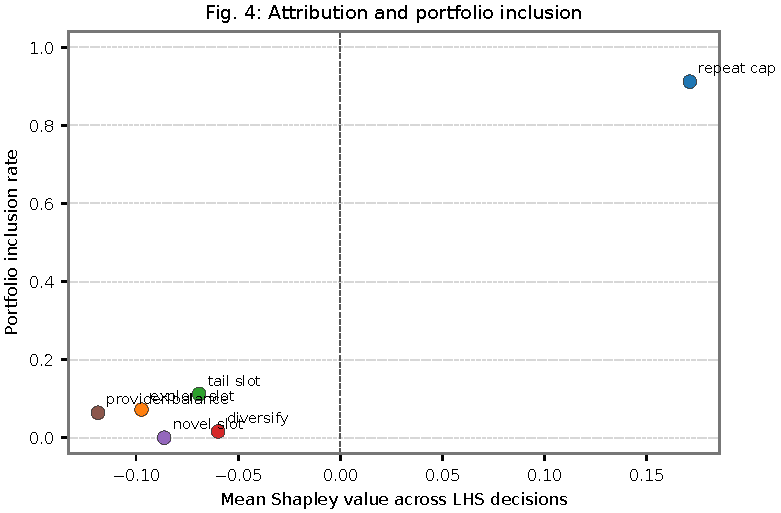
\includegraphics[width=0.88\linewidth]{figures/figure_04_attribution_decision.pdf}
\caption{Design-level attribution and inclusion summary over the 125 LHS games. The horizontal mean aggregates heterogeneous games and can hide configuration-level sign reversals; it is not an attribution for any individual game.}
\label{fig:lhs-stability}
\end{figure}
\FloatBarrier

\section{External evaluation audit}\label{app:audit}
The popularity baseline uses training counts only. BPR-MF optimizes
\begin{equation}
 \mathcal{L}_{\mathrm{BPR}}=-\frac{1}{|\mathcal B|}\sum_{(u,i,j)\in\mathcal B}\log\sigma(x_{ui}-x_{uj}),\qquad x_{ui}=\mathbf z_u^\top\mathbf z_i+\eta_i,
\label{eq:bpr-loss}
\end{equation}
with Adam, $L_2$ weight decay, gradient clipping, and unseen-item negative sampling. SASRec uses causal self-attention over chronological prefixes and the pairwise loss
\begin{equation}
 \mathcal{L}_{\mathrm{SASRec}}=-\frac{1}{|\mathcal B|}\sum_{(u,i^+,j)\in\mathcal B}\log\sigma\!\left(\mathbf s_u^\top\mathbf z_{i^+}+\eta_{i^+}-\mathbf s_u^\top\mathbf z_j-\eta_j\right),
\label{eq:sasrec-loss}
\end{equation}
with AdamW. The selected negative strategy is a $30\%$ uniform, $70\%$ popularity-proportional mixture restricted to unseen training items.

The BPR search first crosses learning rate $\{0.001,0.003,0.01\}$, weight decay $\{10^{-5},10^{-4},10^{-3}\}$, and three negative-sampling strategies at 64 factors; it then refines the top validation configurations over factors $\{32,64,128\}$ and batch sizes $\{2048,4096,8192\}$ before evaluating validation-only popularity hybrids. The selected BPR configuration has 128 factors, batch size 8,192, learning rate $0.003$, weight decay $10^{-5}$, popularity-mixture negatives, and a 200-epoch maximum with early stopping. SASRec is selected independently over embedding dimension, sequence length, attention heads/layers, dropout, batch size, learning rate, weight decay, and negative strategy. Its selected configuration has dimension 128, sequence length 25, two heads, two layers, dropout 0.10, batch size 1,024, learning rate $5\times10^{-4}$, weight decay $10^{-5}$, popularity-mixture negatives, and a 120-epoch maximum with early stopping. Right padding avoids all-masked causal-padding query rows on the tested MPS backend. Full staged-search manifests, epoch budgets, and configuration hashes are retained in the artifact.

For the final SASRec audit, both popularity and SASRec evaluate 1,000 warm targets, count one cold test target, and use candidate sets with mean size 3,436.958 (minimum 2,739; maximum 3,521). Seen-item violations, missing-target violations, candidate-equality violations, and descending-score violations are all zero. SASRec's best validation epoch and restored checkpoint epoch are both 20 for the final audit. The BPR and SASRec seed summaries in the reproducibility snapshot retain all five fixed-seed rows and paired differences against popularity.

As a negative transfer check, MovieLens-25M is evaluated under a separate chronological warm-item protocol using a NumPy BPR fallback that is not implementation-identical to the MovieLens-1M model. On 1,000 paired users it is below popularity by $-0.046$ Hit@10 (95\% paired-user bootstrap CI $[-0.060,-0.033]$, $d_z=-0.219$) and $-0.02040$ NDCG@10 (CI $[-0.02688,-0.01437]$, $d_z=-0.203$). This appendix diagnostic is not a model benchmark and does not support a general claim that BPR is inferior; it is retained to expose an unfavourable transfer result rather than selectively reporting only MovieLens-1M.

\section{Additional diagnostics}\label{app:additional-diagnostics}

\subsection{Ablations and negative evidence}\label{sec:ablations}
The controlled misspecification regime fails oracle recovery as intended; the unstable quick behavioural sweep is excluded from the primary claim; all OAT/LHS configurations are retained; the evaluator records rather than drops the cold target; and the selected SASRec model is not a post-test popularity blend. Seed dispersion describes optimization or simulator variation under the fixed protocols, not population uncertainty over platforms.

\subsection{Selection, approximation, CRN, and scalability}\label{sec:robustness-extensions}
Freezing repeat cap on selection seeds 42--46 and evaluating seeds 200--219 yields held-out lower and upper improvements $0.29235$ and $0.31500$. The maximin-versus-mean and hard-constraint-versus-penalty ablation selects repeat cap for all tested penalty coefficients $\{0,0.25,0.5,1,2,5,10\}$, a null decision result rather than evidence of universal maximin superiority. Sampled six-player attribution has MAE $0.00219$ at budget 32 and $0.00038$ at budget 2048, with unit sign agreement and rank correlation.

The stochastic click-feedback CRN diagnostic uses $w_{\mathrm{click}}=0.35$, seeds 300--319, and coalition pairs $0\to1$ and $1\to5$. Variance ratios are $1.00122$ and $1.00121$, with bootstrap intervals $[0.99763,1.00601]$ and $[0.97816,1.03538]$; no material variance reduction is observed. Table~\ref{tab:integrated-scalability} reports completed rollout-based scaling through $n=8$. The artifact contains an $n=10$ driver, but no completed integrated $n=10$ result is claimed.

\FloatBarrier
\begin{table}[!ht]
\caption{Completed integrated scalability with executable operator semantics (full configuration, seed 42).}\label{tab:integrated-scalability}
\centering
\scriptsize
\setlength{\tabcolsep}{3pt}
\begin{tabular}{@{}lrrrrlr@{}}
\toprule
Players & Coal. & Time (s) & Peak MB & Eff. gap & Decision (lower) & Regret\\
\midrule
$n=6$ & 64 & 1,804 & $\leq$114 & 0 & repeat cap (repair), $0.298514$ & 0\\
$n=8$ & 256 & 7,505 & 114 & 0 & repeat cap (repair), $0.298514$ & 0\\
\bottomrule
\end{tabular}
\end{table}
\FloatBarrier

\subsection{Learned base policy inside the intervention game}\label{sec:semireal}
Under the full configuration and seed 42, a BPR-MF ranker (32 factors, 60,000 updates) is fitted to 14,400 simulator-logged impressions and substituted for the hand-crafted base without changing scenarios, interventions, constraints, or seeds. Table~\ref{tab:semireal} shows that this single integration case remains in repair mode and selects repeat cap; it does not establish general consistency across learned policies or real logs.

\FloatBarrier
\begin{table}[!ht]
\caption{Learned-base-policy integration (seed 42, full configuration).}\label{tab:semireal}
\centering
\scriptsize
\setlength{\tabcolsep}{3pt}
\begin{tabularx}{\linewidth}{@{}Xllrrrr@{}}
\toprule
Base policy & Mode & Selected & Lower & Upper & Disparity upper & Relevance $\Delta$\\
\midrule
Hand-crafted & repair & repeat cap & 0.298514 & 0.313069 & 0.225872 & $-0.044137$\\
Simulator-trained BPR & repair & repeat cap & 0.335378 & 0.369736 & 0.181806 & $-0.050223$\\
\bottomrule
\end{tabularx}
\end{table}
\FloatBarrier

\section{Claim boundaries}\label{app:claims}
The following claims are supported by the corresponding evidence.
\begin{itemize}
\item \textbf{Controlled causal claim:} exact-game recovery and misspecification behaviour are established within the analytic and behavioural \Sim{} mechanisms.
\item \textbf{Behavioural robustness claim:} the reported OAT and LHS selection frequencies, utility summaries, repairs, and switches hold for the disclosed finite configurations and seeds.
\item \textbf{External ranking claim:} BPR and SASRec produce the reported chronological warm-item ranking metrics under the shared MovieLens evaluator.
\item \textbf{Unsupported claim:} no result in this artifact identifies the long-run causal effect of a policy intervention from MovieLens ratings alone.
\end{itemize}

\section{CURE-Sim structural mechanisms}\label{app:scm}
For user $u$, item $j$, and slate position $\ell\in\{0,\ldots,k-1\}$ (zero-indexed), the simulator uses normalized latent item vector $e_j\in\mathbb{R}^d$, hidden user interest $h_{u,t}\in\mathbb{R}^d$ at time $t$, public profile $p_u\in\mathbb{R}^d$, item base quality $a_j\in\mathbb{R}$, exposure count $E_{uj,t}\in\mathbb{N}$, user fatigue $F_{u,t}\in[0,1]$, and item popularity $Q_{j,t}\in\mathbb{R}_{\geq0}$. The latent interest evolves over time, so every mechanism below conditions on $h_{u,t}$, not on a frozen vector. With $r$ the repeat threshold, the repeated-item indicator is $z_{uj,t}=\mathbf{1}\{E_{uj,t}\ge r\}$. The response probability is
\begin{equation}
 \begin{aligned}
 \Pr(Y_{uj\ell t}=1)=\sigma\!\biggl(&1.6 e_j^\top h_{u,t}
 +\frac{0.45}{\sqrt{\ell+1}}+0.15\log(1+Q_{j,t})\\[-2pt]
 &{}-0.85\,\alpha_m F_{u,t}-0.55z_{uj,t}+\delta_m\biggr),
 \end{aligned}
\label{eq:response}
\end{equation}
where $\alpha_m$ and $\delta_m$ are the declared scenario fatigue multiplier and satisfaction shift (multiplied by the baseline fatigue multiplier, equal to one in the full configuration). Item satisfaction and relevance for the displayed slate are respectively $\sigma(1.8e_j^\top h_{u,t}-0.7z_{uj,t}-0.4F_{u,t})$ and $\sigma(1.7e_j^\top h_{u,t}+a_j)$, averaged over the slate at each step. The update equations are
\begin{align}
 E_{uj,t+1}&=E_{uj,t}+\mathbf{1}\{j\in L_{u,t}\},\label{eq:exposure}\\
 G_{g,t+1}&=G_{g,t}+\sum_{u\in\mathcal U}\sum_{j\in L_{u,t}}\mathbf{1}\{\mathrm{prov}(j)=g\},\label{eq:provider-exposure}\\
 F_{u,t+1}&=\mathrm{clip}\{0.88F_{u,t}+0.22\,\overline z_{u,t},0,1\},\label{eq:fatigue-update}\\
 Q_{j,t+1}&=Q_{j,t}+\beta_m\rho\,\sum_{u\in\mathcal U}\mathbf{1}\{j\in L_{u,t}\},\label{eq:popularity}\\
 h_{u,t+1}&=\mathrm{norm}\{h_{u,t}+0.03\,\overline f_{u,t}\,\overline e_{u,t}+\nu\,\overline e^{\mathrm{novel}}_{u,t}\}.\label{eq:interest}
\end{align}
At each time step the implementation performs the operations in this order: (1) score the eligible candidates with the base ranker; (2) apply the coalition's canonical slate transformations; (3) compute satisfaction and draw response outcomes; (4) update user--item and provider exposure; (5) update fatigue; (6) update popularity; and (7) update latent interest. All updates use the displayed slate and the pre-update state for that step. Stating this order is necessary because alternative within-step orderings can produce different trajectories.

The barred quantities are explicit slate aggregates over $L_{u,t}$: $\overline z_{u,t}=k^{-1}\sum_{j\in L_{u,t}}z_{uj,t}$ is the slate repeat rate; $\overline e_{u,t}=k^{-1}\sum_{j\in L_{u,t}}e_j$ is the mean displayed item feature; $\overline f_{u,t}$ is the feedback signal $(1-w_{\mathrm{click}})\,\overline s_{u,t}+w_{\mathrm{click}}\,\overline c_{u,t}$, where $\overline s_{u,t}$ is the slate-mean satisfaction, $\overline c_{u,t}$ the slate click rate, and $w_{\mathrm{click}}=0$ in the primary configuration; and the novelty direction is
\begin{equation}
 \overline e^{\mathrm{novel}}_{u,t}=\frac{\sum_{j\in L_{u,t}}[-e_j^\top p_u]_+\,e_j}{\max\{\sum_{j\in L_{u,t}}[-e_j^\top p_u]_+,\,10^{-8}\}},
\end{equation}
computed only over displayed items with negative public-profile similarity. If no displayed item has negative similarity, or when $\nu=0$ as in the archived baseline, the novelty term in Eq.~\eqref{eq:interest} is identically zero. $\mathrm{norm}$ renormalizes to unit Euclidean norm.

In the primary configuration, $w_{\mathrm{click}}=0$, so realized binary clicks are retained as simulated response outcomes but do not enter the preference-drift feedback signal; drift is driven by slate-mean satisfaction. The separate common-random-number diagnostic activates click feedback with $w_{\mathrm{click}}=0.35$.

Exposure accounting in Eq.~\eqref{eq:exposure} counts every displayed slate item independently of whether it was clicked; provider exposure in Eq.~\eqref{eq:provider-exposure} and the popularity update in Eq.~\eqref{eq:popularity} are likewise impression-based. The popularity increment intentionally grows with cohort size: with $\rho=0.025$ and scenario multiplier $\beta_m$, each display adds $\beta_m\rho$ to $Q_{j,t}$, so aggregate popularity is proportional to cohort impressions rather than normalized by $|\mathcal{U}|$. This is a disclosed scaling choice of the simulator, not a platform-invariance claim. Provider disparity is the Gini coefficient of terminal cumulative provider exposure $x=G_T\in\mathbb{R}_{\geq0}^{|\mathcal{P}|}$. For components sorted as $x_{(1)}\leq\cdots\leq x_{(|\mathcal{P}|)}$, it is
\begin{equation}
 d=\frac{2\sum_{i=1}^{|\mathcal{P}|}i\,x_{(i)}}{|\mathcal{P}|\sum_{i=1}^{|\mathcal{P}|}x_{(i)}}-\frac{|\mathcal{P}|+1}{|\mathcal{P}|},
\label{eq:gini}
\end{equation}
with $d=0$ by convention when all providers have zero exposure. The base ranker scores $e_j^\top p_u+\lambda_{\mathrm{pop}}\log(1+Q_{j,t})$ with profile weight $1.0$ and popularity weight $\lambda_{\mathrm{pop}}=0.30$ in the full configuration, breaking score ties by ascending item identifier. These equations define the simulator characteristic function conditional on the configuration; they are not claimed to be a fitted structural model of MovieLens.

\section{Scenario and calibration protocol}\label{app:protocol}
The full behavioural configuration fixes 120 users, 240 items, 18 providers, 10 categories, 12 latent dimensions, a 12-step horizon, and slate size 10. Table~\ref{tab:scenarios} lists every numerical scenario parameter. The effective fatigue multiplier in Eq.~\eqref{eq:response} is the product of the baseline fatigue multiplier ($1.0$) and the scenario multiplier $\alpha_m$; the popularity increment per display is $\beta_m\rho$ with baseline popularity feedback $\rho=0.025$; the click-feedback weight $w_{\mathrm{click}}$ is $0$ in every primary scenario; and the novelty-drift coefficient is $\nu=0$ in the baseline. The intervention costs used in the full configuration are 0.05 for repeat cap, 0.10 for exploration, 0.08 for long-tail, 0.06 for diversity, 0.08 for novelty, and 0.12 for provider balancing, giving $c(\Players)=0.49$. The budget is 0.35, the minimum relevance change is $-0.08$, the maximum provider disparity is 0.28, and maximum fatigue is 0.65. The utility parameters are $\gamma=0.97$ and $(w_s,w_r,w_f,w_c)=(0.70,0.30,0.35,1.00)$.

\begin{table}[h]
\caption{Complete numerical scenario specification of the full CURE-Sim configuration. All values are pre-specified; none is tuned after observing outcomes.}\label{tab:scenarios}
\centering
\small
\setlength{\tabcolsep}{5pt}
\begin{tabular}{@{}lcccc@{}}
\toprule
Scenario & Fatigue mult.\ $\alpha_m$ & Popularity mult.\ $\beta_m$ & Satisfaction shift $\delta_m$ & $w_{\mathrm{click}}$\\
\midrule
nominal & 1.00 & 1.00 & $0.00$ & 0\\
fatigue\_stress & 1.40 & 1.00 & $-0.03$ & 0\\
popularity\_stress & 1.00 & 1.75 & $-0.02$ & 0\\
mixed\_stress & 1.30 & 1.50 & $-0.04$ & 0\\
\bottomrule
\end{tabular}
\end{table}

The OAT protocol retains the baseline and changes one assumption at a time. It evaluates fatigue strengths 0.75 and 1.25; repeat thresholds 2 and 4; horizons 8 and 16; provider thresholds 0.24 and 0.32; provider-balance strengths 0.15 and 0.55; novelty preference drift 0.03 and 0.06; and exploration costs 0.05 and 0.15. The LHS protocol samples 24 joint settings over the declared ranges plus the baseline. The declared joint ranges are: fatigue strength $[0.70,1.40]$; repeat threshold $\{1,\ldots,5\}$; horizon $\{4,\ldots,20\}$; provider threshold $[0.20,0.36]$; provider-balance strength $[0.0,0.80]$; novelty delayed benefit $[0.0,0.08]$; and exploration cost $[0.02,0.20]$. Both protocols use seeds 42--46. No setting is selected as the reported primary configuration after observing utility; all are retained in the archived configuration tables.

\section{External fixed-seed results}\label{app:external-seeds}
Table~\ref{tab:sas-seeds} reports every frozen SASRec replication used in the five-seed summary.
\begin{table*}[t]
\caption{Frozen SASRec seed replication under the shared MovieLens warm-item evaluator.}\label{tab:sas-seeds}
\centering
\scriptsize
\setlength{\tabcolsep}{2pt}
\resizebox{\textwidth}{!}{%
\begin{tabular}{@{}rrrrrr@{}}
\toprule
Seed & SASRec $\Recall$ & SASRec $\NDCG$ & Popularity $\Recall$ & Popularity $\NDCG$ & Best epoch\\
\midrule
42 & 0.145 & 0.075122 & 0.049 & 0.025520 & 20\\
43 & 0.146 & 0.074018 & 0.049 & 0.025520 & 48\\
44 & 0.140 & 0.071049 & 0.049 & 0.025520 & 42\\
45 & 0.147 & 0.078446 & 0.049 & 0.025520 & 44\\
46 & 0.148 & 0.072547 & 0.049 & 0.025520 & 60\\
\bottomrule
\end{tabular}}
\end{table*}

The selected final BPR configuration uses hash \texttt{9875430c235b}; the selected SASRec configuration uses hash \texttt{7aa511398a7f}. Each seed replication checks that the configuration hash matches the frozen search manifest before its metric row is accepted. This prevents a stale result directory from being silently mixed with a later configuration.

%% Rendered with an explicit letter to avoid a numbering artifact observed in
%% earlier builds (``9 Artifact inventory''); this section is not cross-referenced.
\section*{Appendix I --- Artifact inventory}\label{app:artifacts}
The reproducibility snapshot is intentionally small enough to inspect. It contains the external data-analysis manifest and evaluator tables; BPR staged-search and final-audit files; SASRec final configuration, evaluation audit, pairwise audit, loss, validation, seed metrics, paired metrics, and summary; controlled-regime manifest, selections, attributions, interactions, and figure; and OAT/LHS manifests, configurations, summaries, seed decisions, attributions, interactions, and figures. It omits raw MovieLens data and large model checkpoints. The archive manifest explains how to regenerate those omitted artifacts from the source repository. The decision-focused experiments reported in Sections~\ref{sec:divergent-selectors},~\ref{sec:objective-sensitivity}, and~\ref{sec:semireal} are archived under \texttt{code/results/reviewer\_phase\_assets/} with their own manifests and checksums. Compute-intensive drivers are gathered in \texttt{code/notebooks/13\_reviewer\_closure\_runs.ipynb}; completed outputs are claimed only where corresponding snapshot files have been verified, and the integrated $n=10$ run is not presented as completed.

\end{appendices}

\bibliographystyle{elsarticle-num}
\bibliography{cure-rec-bibliography}

\end{document}
